\subsection{Overview}
The BBP user interface is designed to be simple and easy to use, with a strong focus on map-based features. The system comes with two interface options: a responsive web app built with Vue.js and a native mobile app developed in Flutter. \\
The web application can be accessed from any modern browser and automatically adapts to the device’s screen size. It is mainly intended for viewing routes, managing personal data, and checking trip statistics. \\
The mobile app builds on the web version by adding features that are specific to smartphones. In particular, it uses GPS to record trips in real time and relies on the device’s sensors (accelerometer and gyroscope) to automatically detect obstacles while cycling. \\
Both versions share the same design principles: simplicity of use, focus on geographic visualization through Mapbox maps, and a clear organization of information. The maps are the central element of the user experience, allowing the available routes, the reported obstacles and the recorded trips to be visualized directly on a geographic representation of the territory.

\subsection{Web Application}
The BBP web application provides a complete interface for the management of all aspects of the system. The pages are organized in a coherent way, with a side navigation bar that is always visible and allows moving quickly between the different sections.

\subsubsection{Bike Path Finder}
The Bike Path Finder section is the main tool for discovering new routes. The interface presents a full-screen map on the right side and a scrollable sidebar on the left side that can be opened and closed. The side panel contains a form where the user enters an origin and destination address, selecting for each one a search radius through dropdown menu, with the "Clear" and "Search" buttons to reset or start the search. The results appear as clickable cards that show the addresses, a score, the total distance and the status of the route. Selecting a card, the route is drawn on the map with markers for origin and destination, including any obstacles along the path.
\begin{figure}[h!]
    \centering
        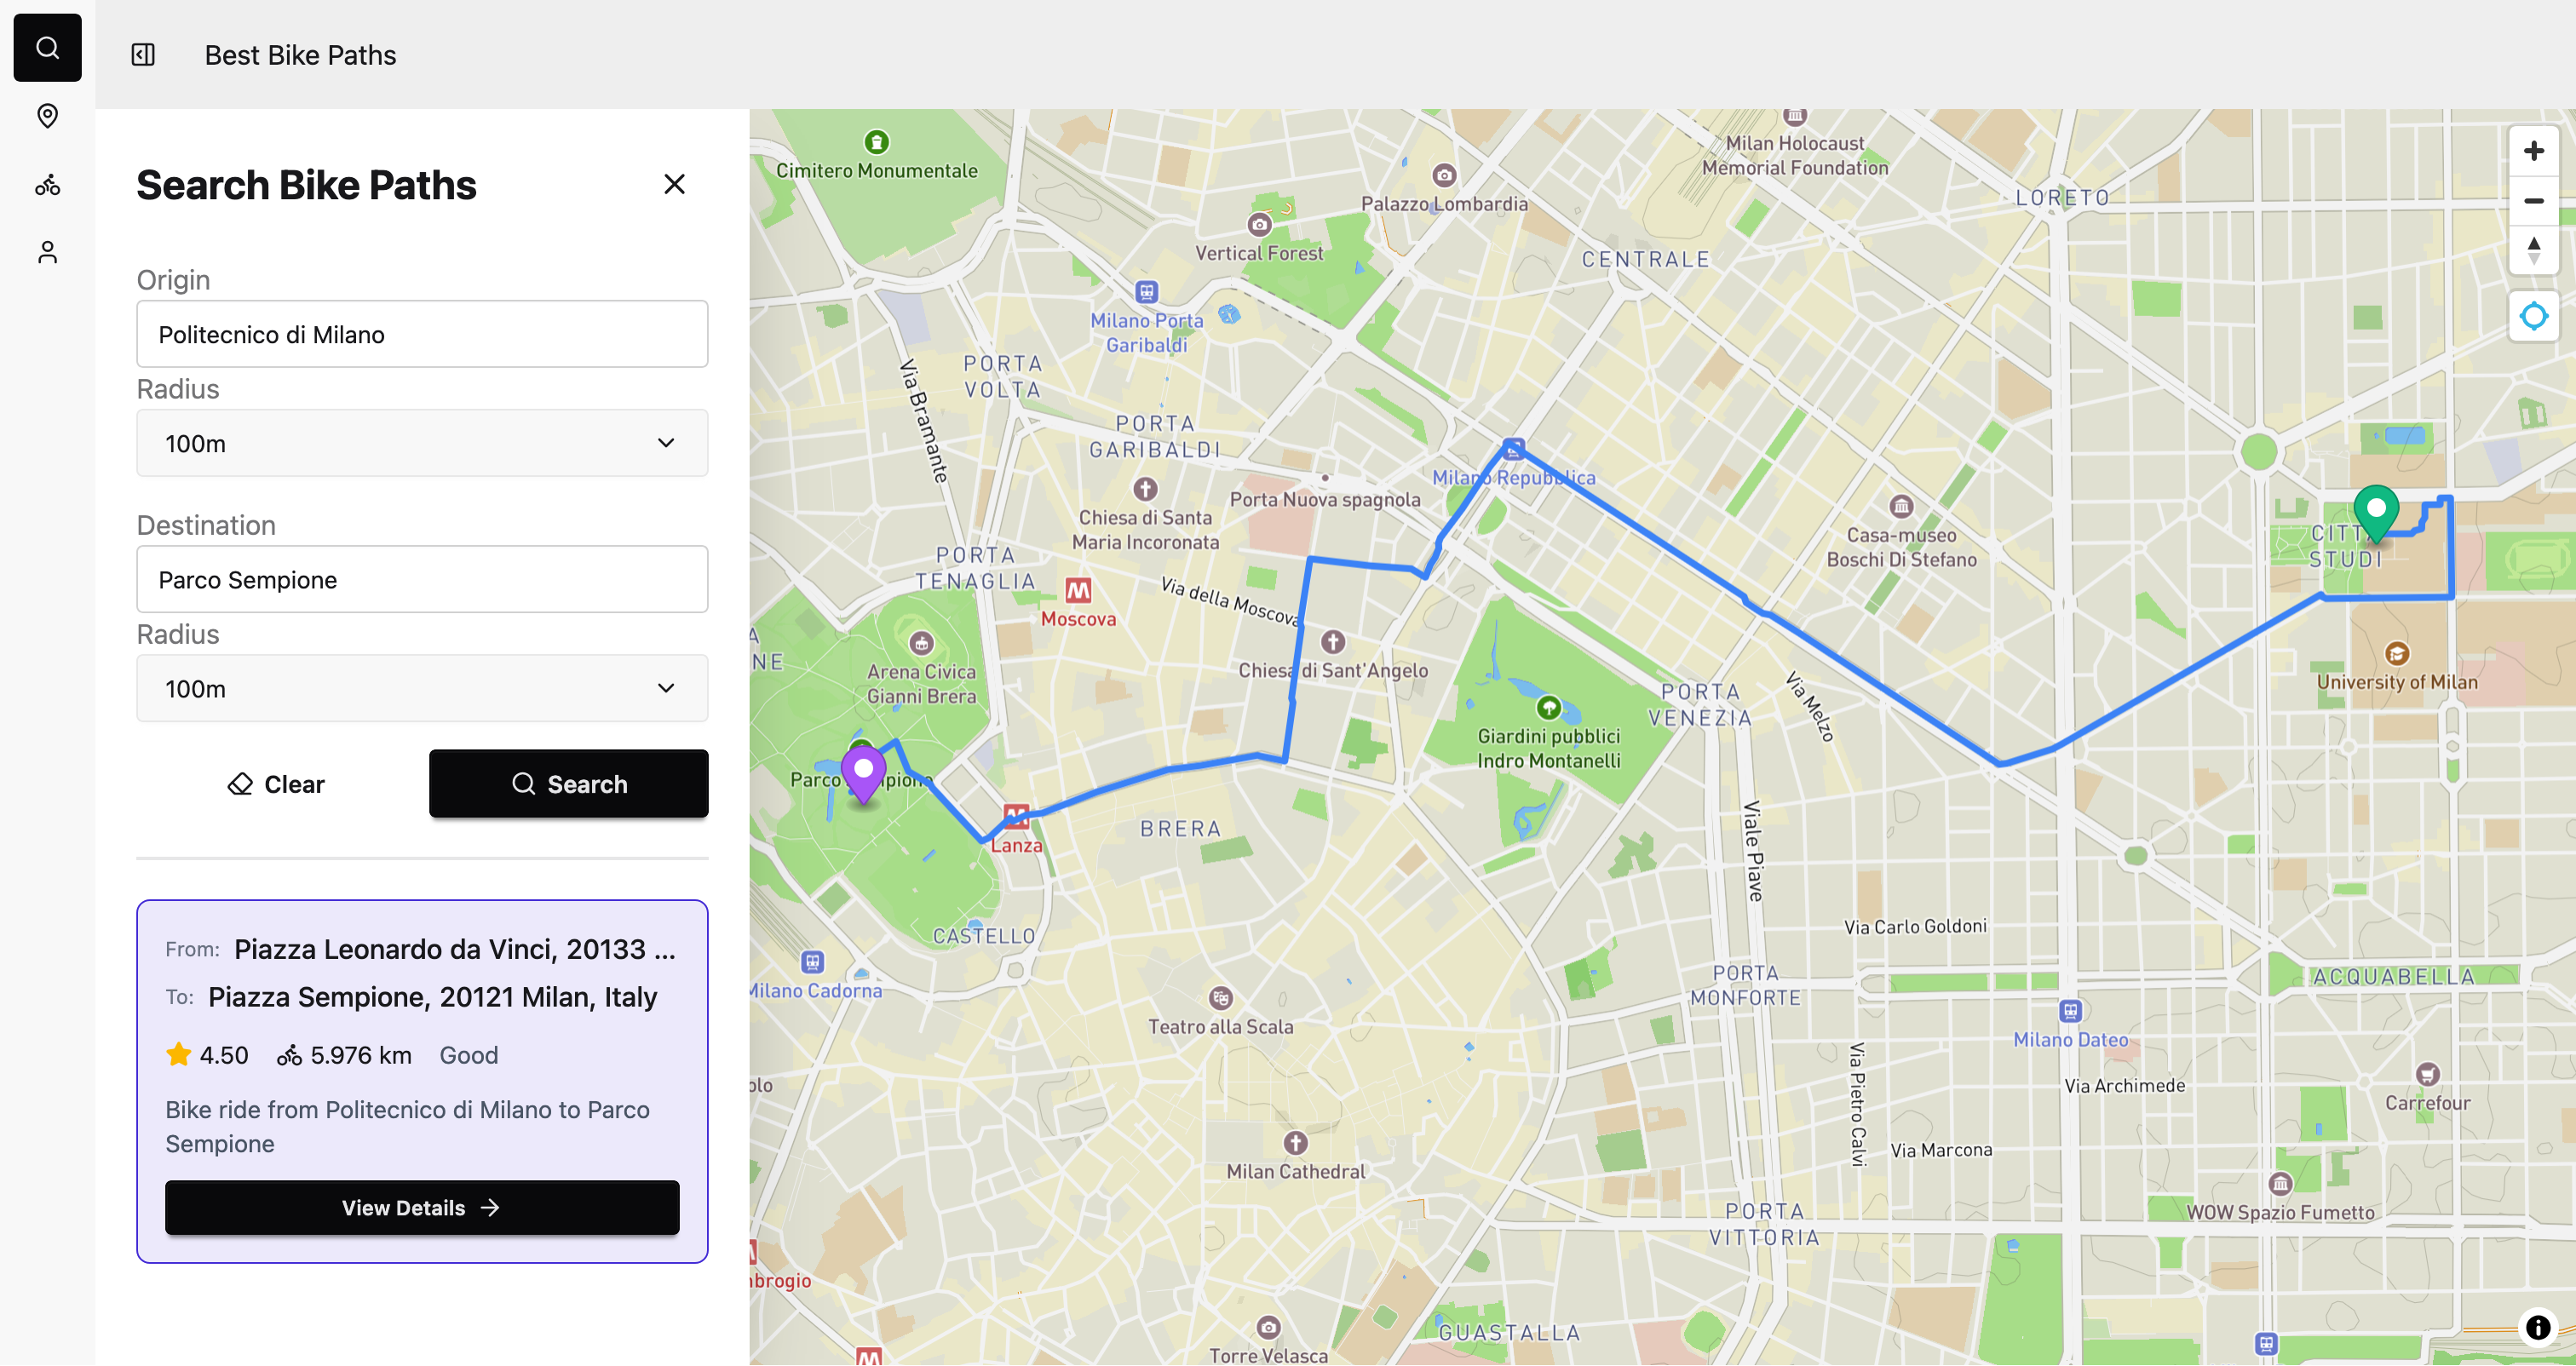
\includegraphics[width=\linewidth]{DD/images/ui-finder.png}
    \caption{Bike Path Finder}
    \label{fig:ui-finder}
\end{figure}

\subsubsection{Trips Management}
The Trips section allows managing the registered bicycle trips through three main views. The Trips view shows a grid of cards with map thumbnails for each route, indicating origin, destination, distance, duration and time interval. The "Filters" and "Record Trip" buttons in the header allow filtering the results by origin, destination and time period, or creating new trips. Selecting a card, one accesses TripDetail which presents an interactive map with the complete route and markers, followed by the trip information including times, average and maximum speed, optional description and meteorological data if available. The TripCreateManual view allows manually recording completed trips through a form that includes a reference map, fields to enter origin addresses, destination and optional waypoints, start and end times, description and optional maximum speed. Users can navigate between the views maintaining the context and use the "Cancel" and "Record" buttons to save or discard the recordings.
\begin{figure}[h!]
    \centering
        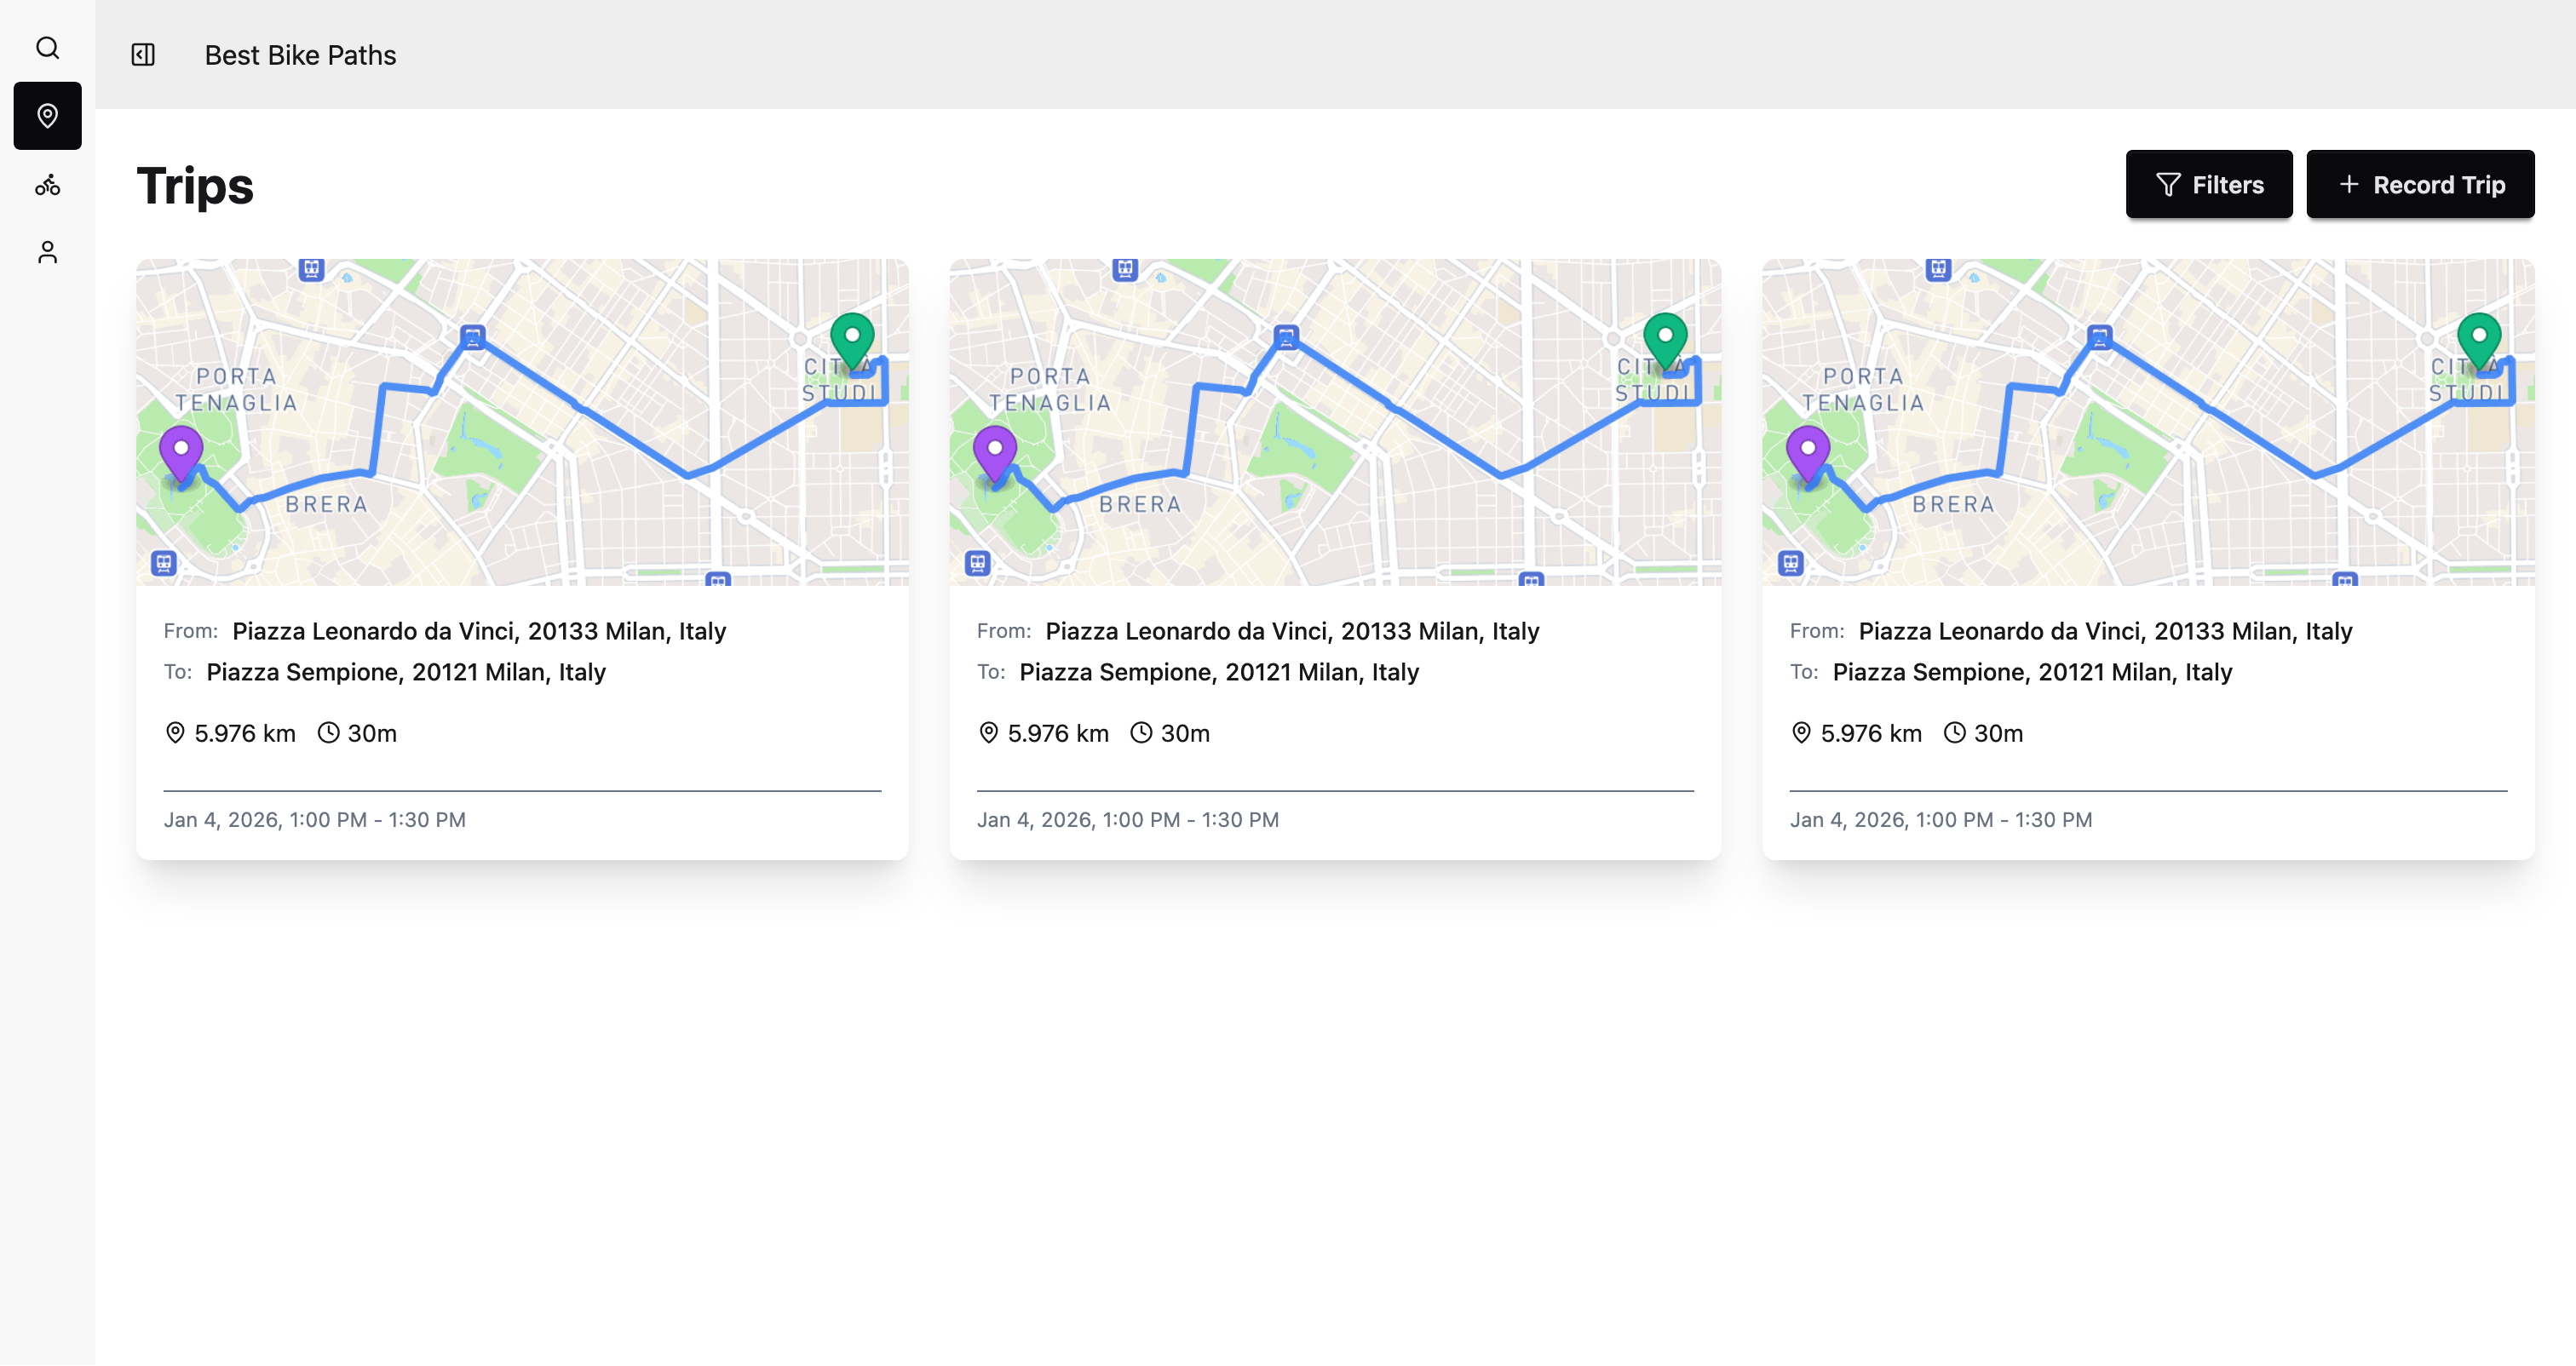
\includegraphics[width=\linewidth]{DD/images/ui-trips.png}
    \caption{Trips}
    \label{fig:ui-trips}
\end{figure}
\begin{figure}[h!]
    \centering
        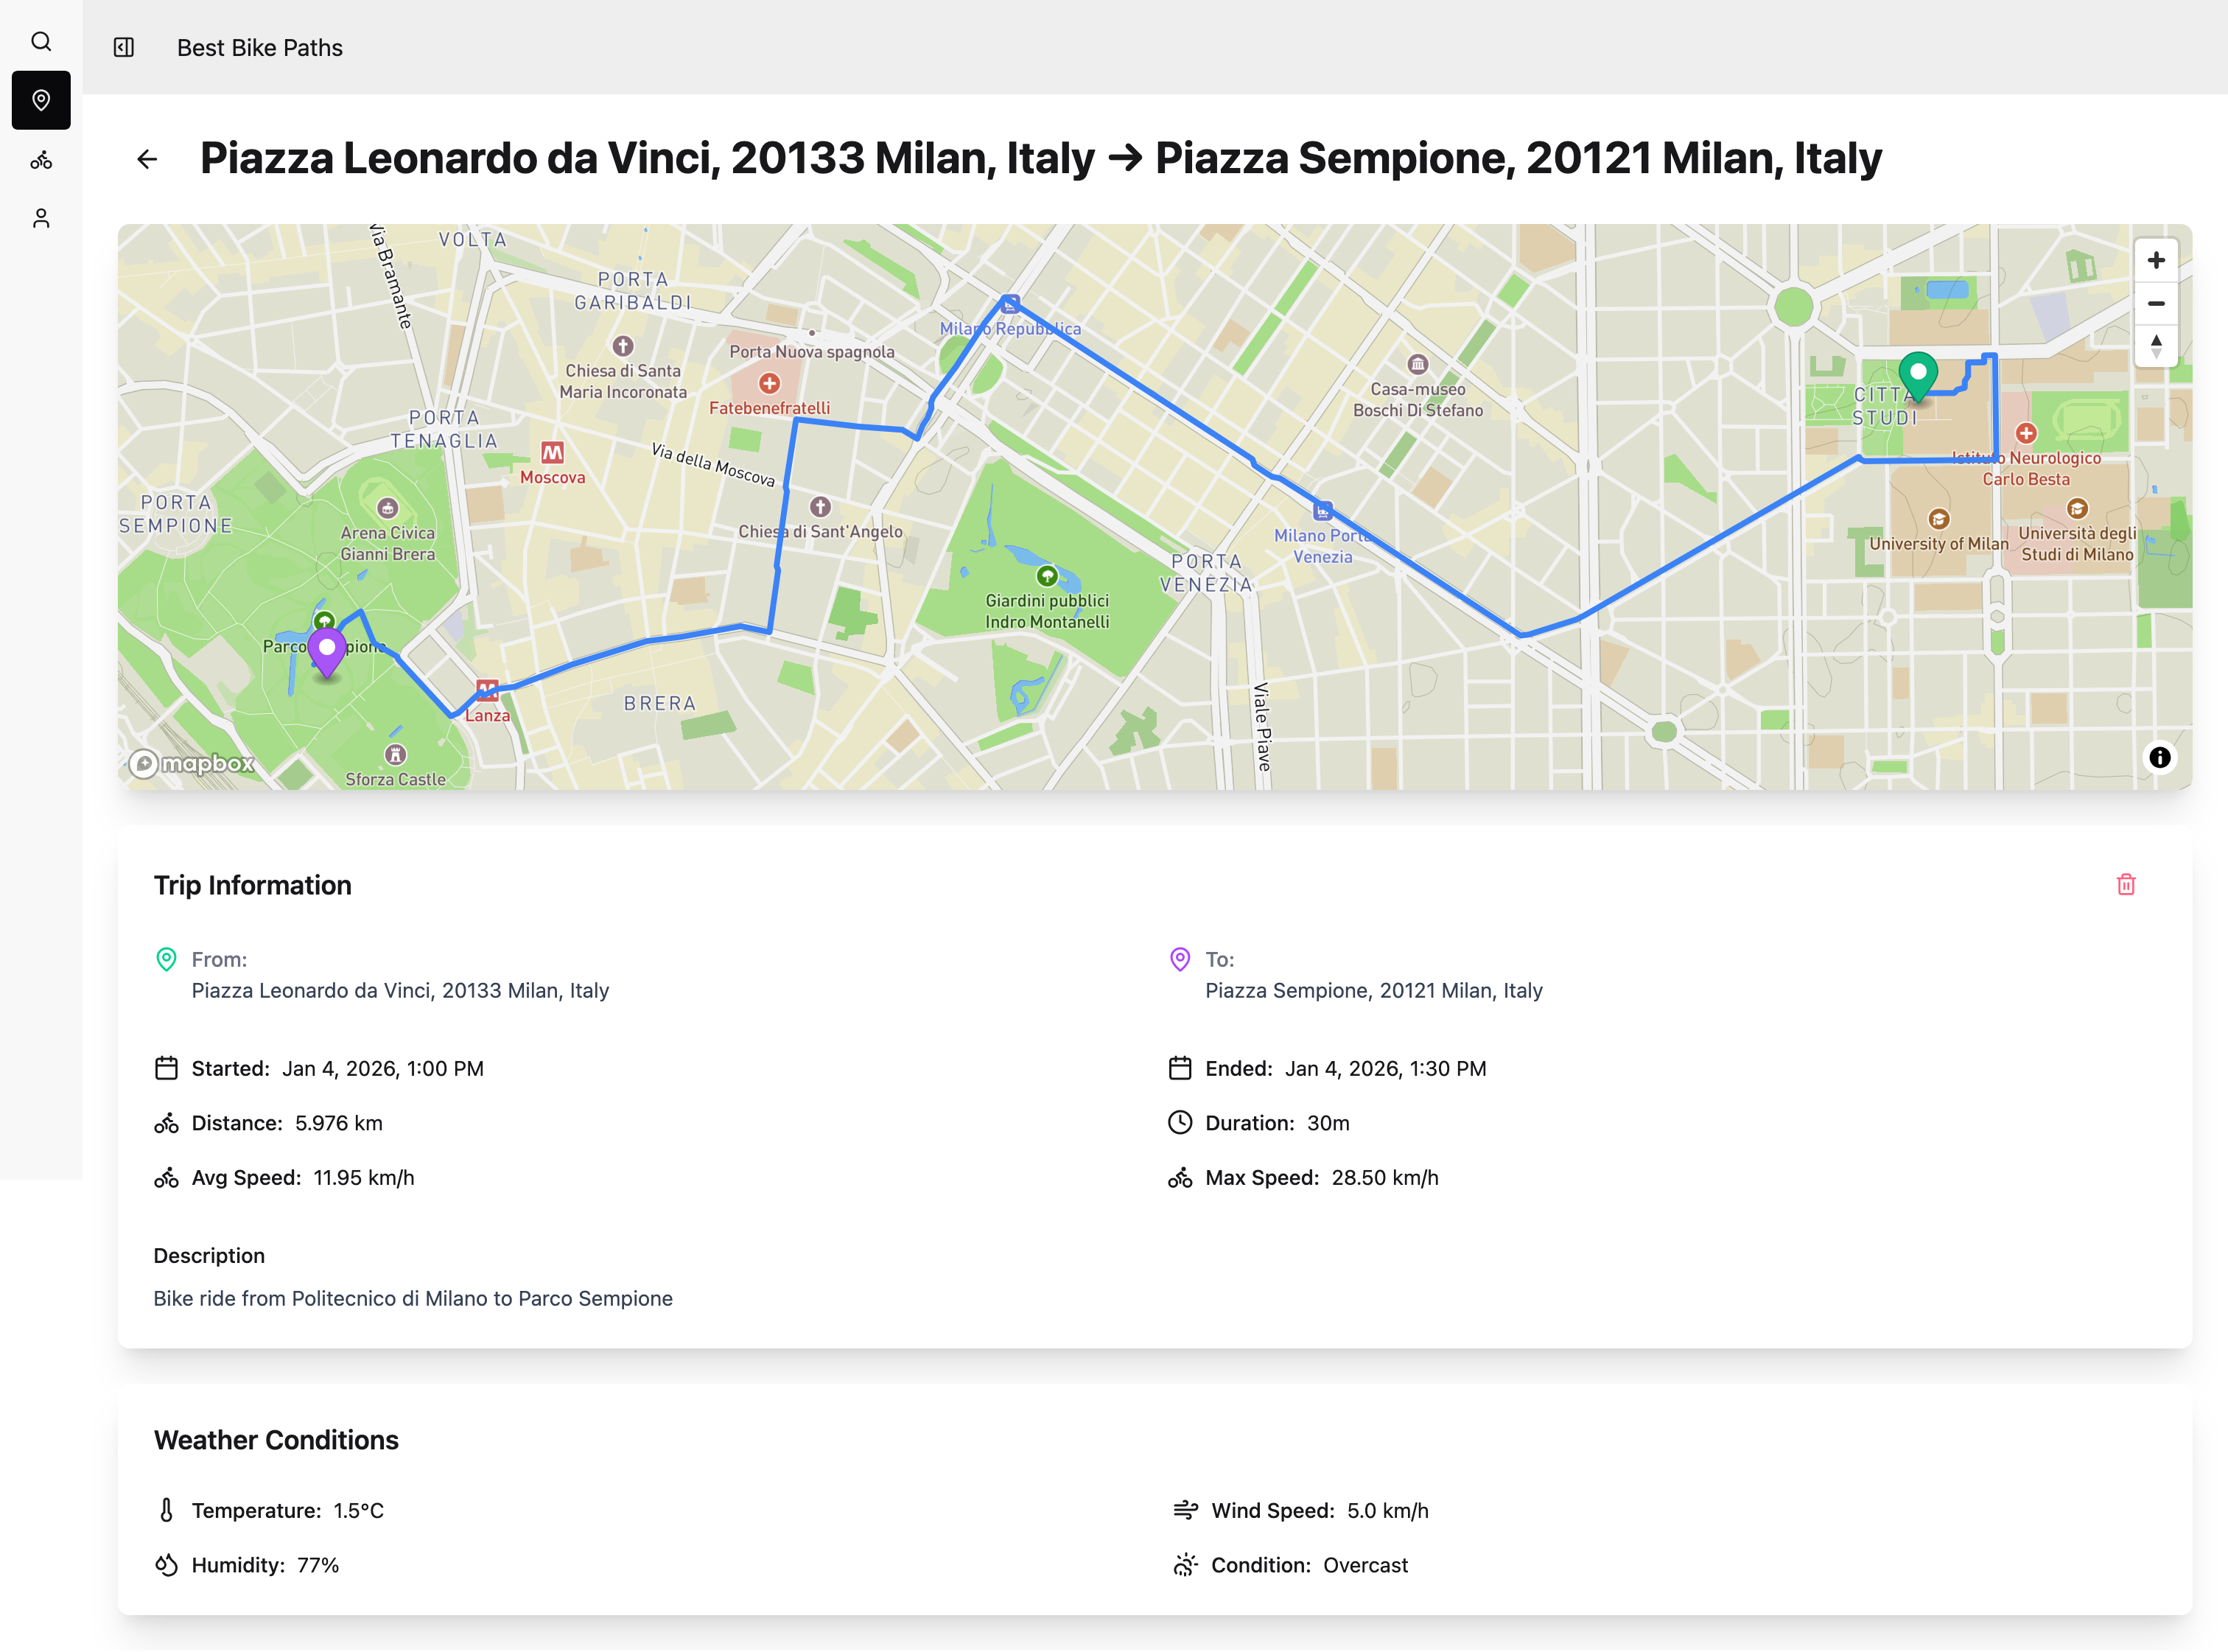
\includegraphics[width=\linewidth]{DD/images/ui-trip-detail.png}
    \caption{Trip Detail}
    \label{fig:ui-trip-detail}
\end{figure}
\begin{figure}[h!]
    \centering
        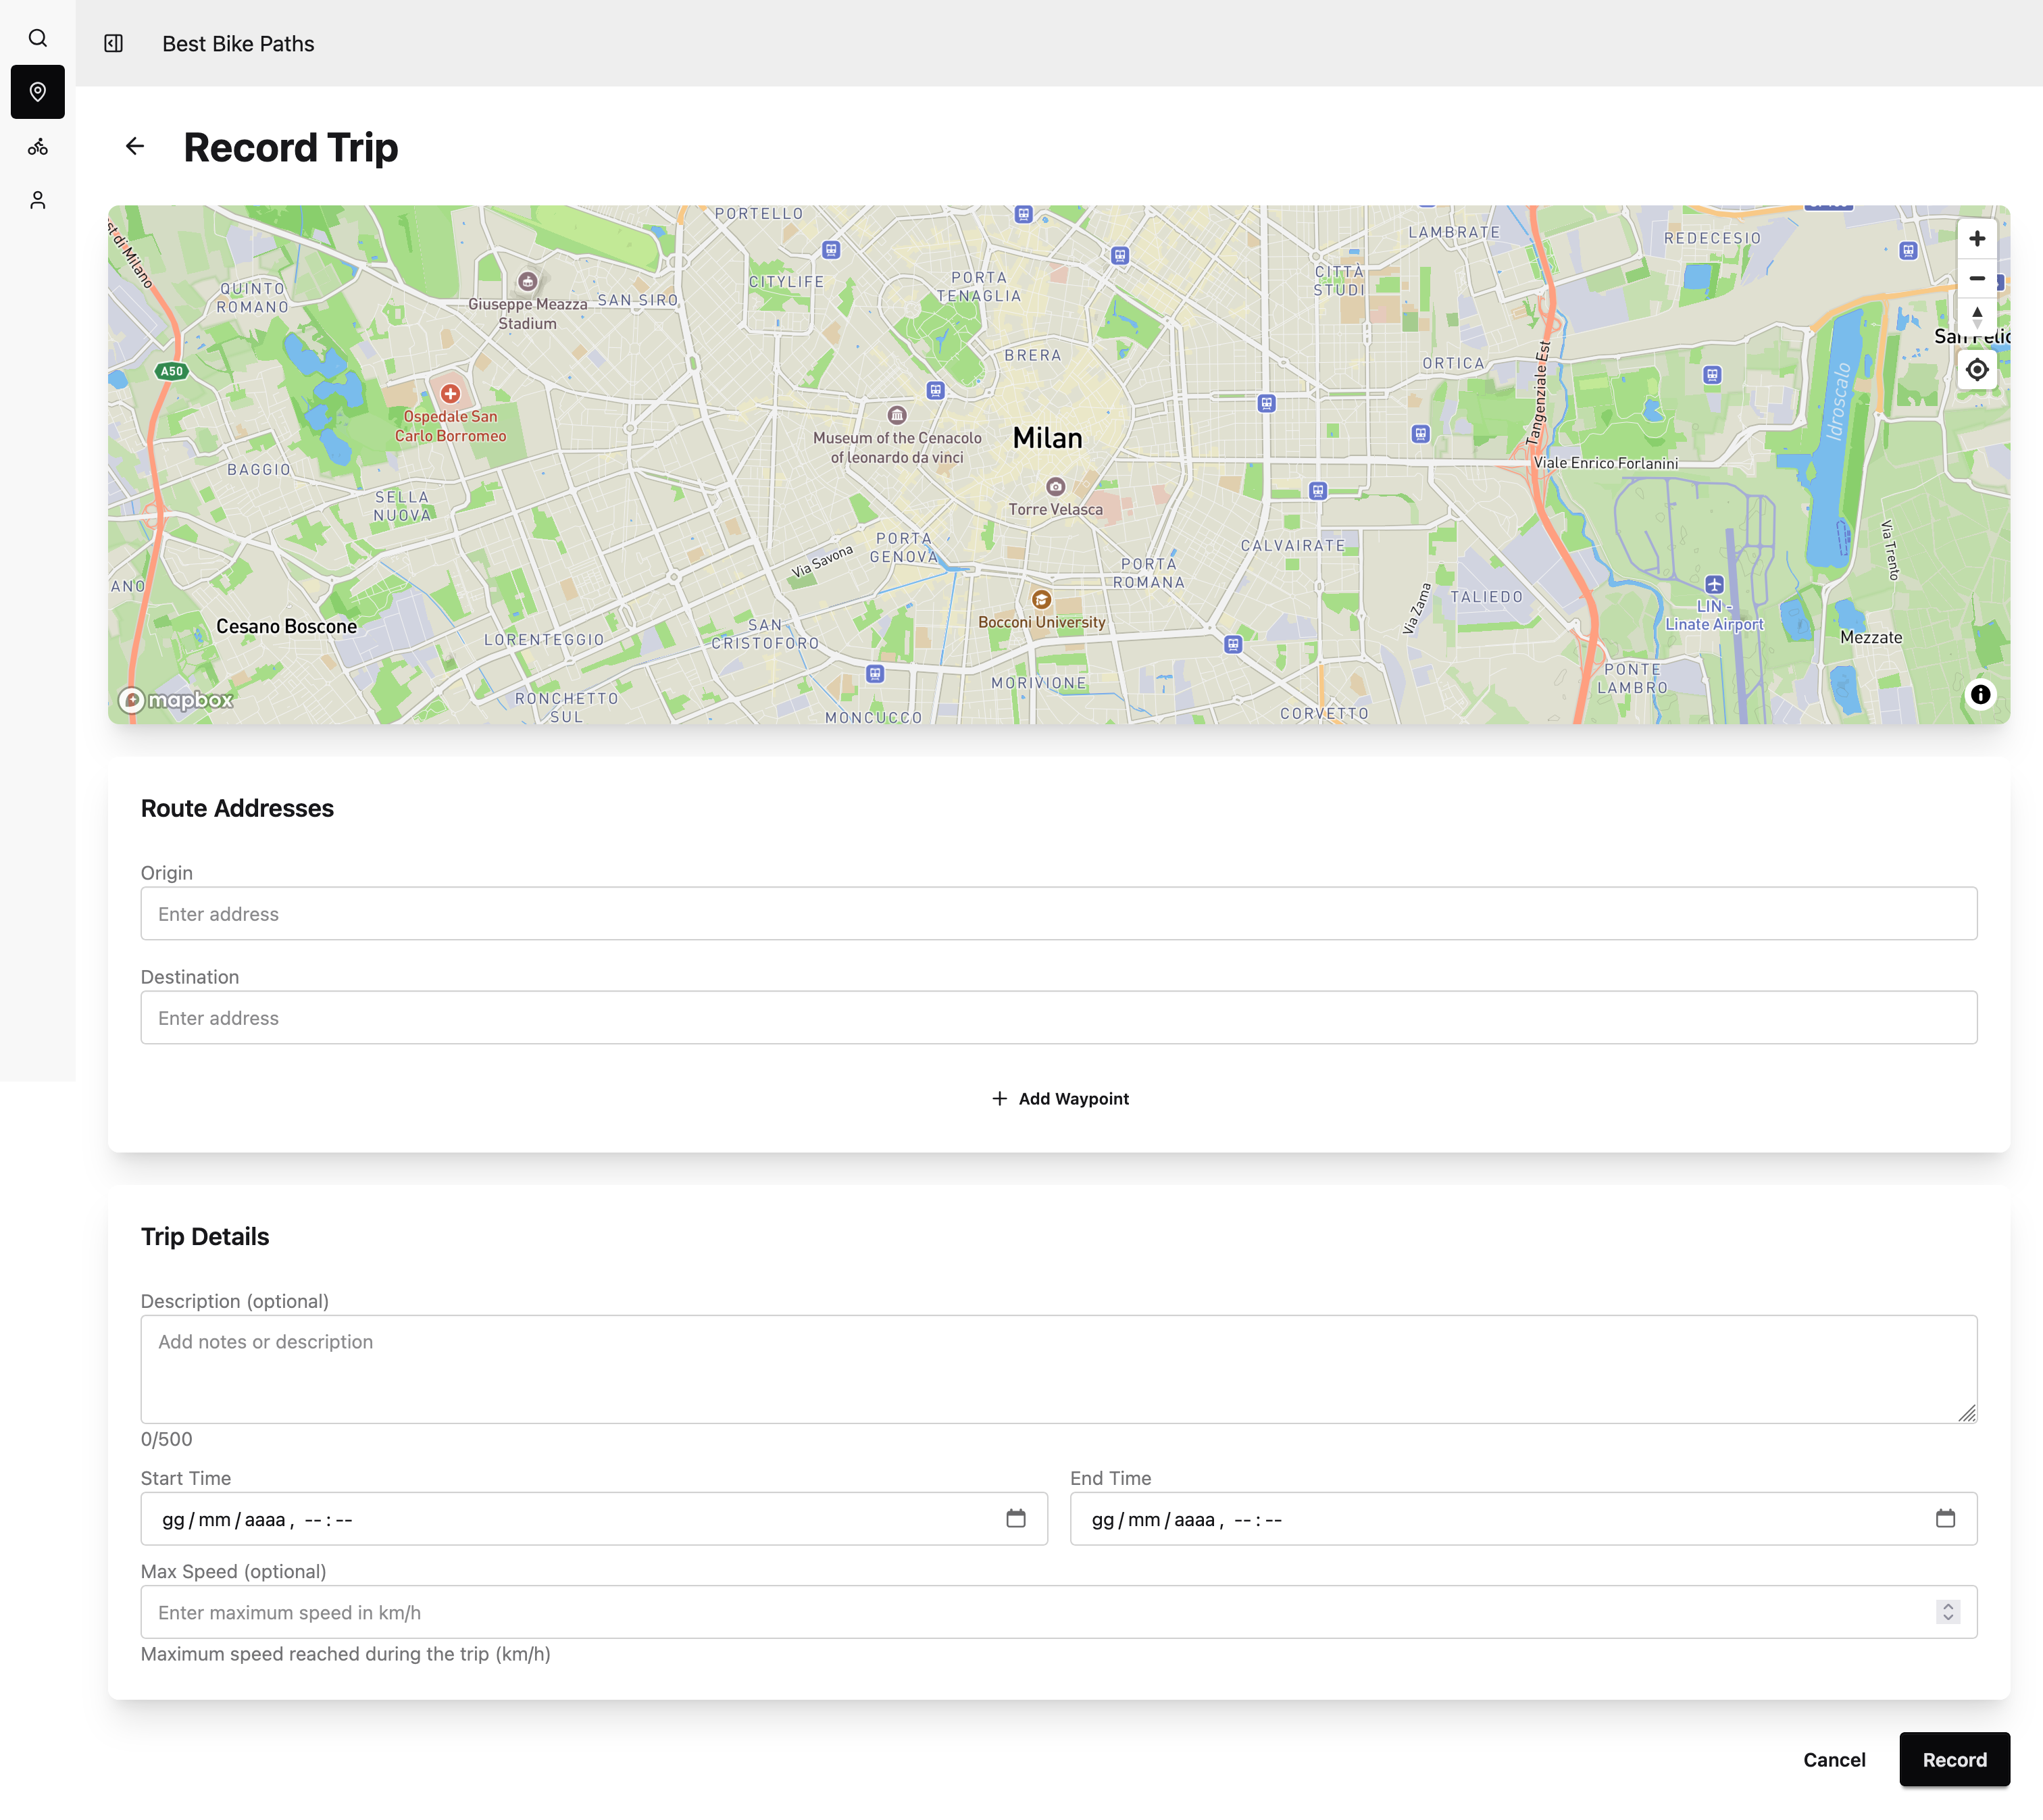
\includegraphics[width=\linewidth]{DD/images/ui-create-trip.png}
    \caption{Trip Create Manual}
    \label{fig:ui-create-trip}
\end{figure}

\subsubsection{Bike Paths Management}
The Bike Paths section allows managing the created cycling routes through three main views. The BikePaths view shows a grid of cards with map thumbnails for each route, indicating origin, destination, score, distance, status and public or private visibility. The "Filters" and "Create Bike Path" buttons in the header allow filtering the results by origin, destination and creation date, or creating new routes. Selecting a card, one accesses BikePathDetail which presents an interactive map with the complete route and markers, followed by the route information including score, distance, status, visibility, editable description and creation/update metadata. The obstacles section shows all the obstacles present on the route with possibility to modify them individually (type, severity, active/inactive status). The BikePathCreateManual view allows manually creating new routes through a form that includes a reference map, fields to enter origin addresses, destination and optional waypoints, description, route status, checkbox to make the route public and an optional section to add obstacles with address, type and severity. Users can navigate between the views maintaining the context and use the "Cancel" and "Create" buttons to save or discard the creations.
\begin{figure}[h!]
    \centering
        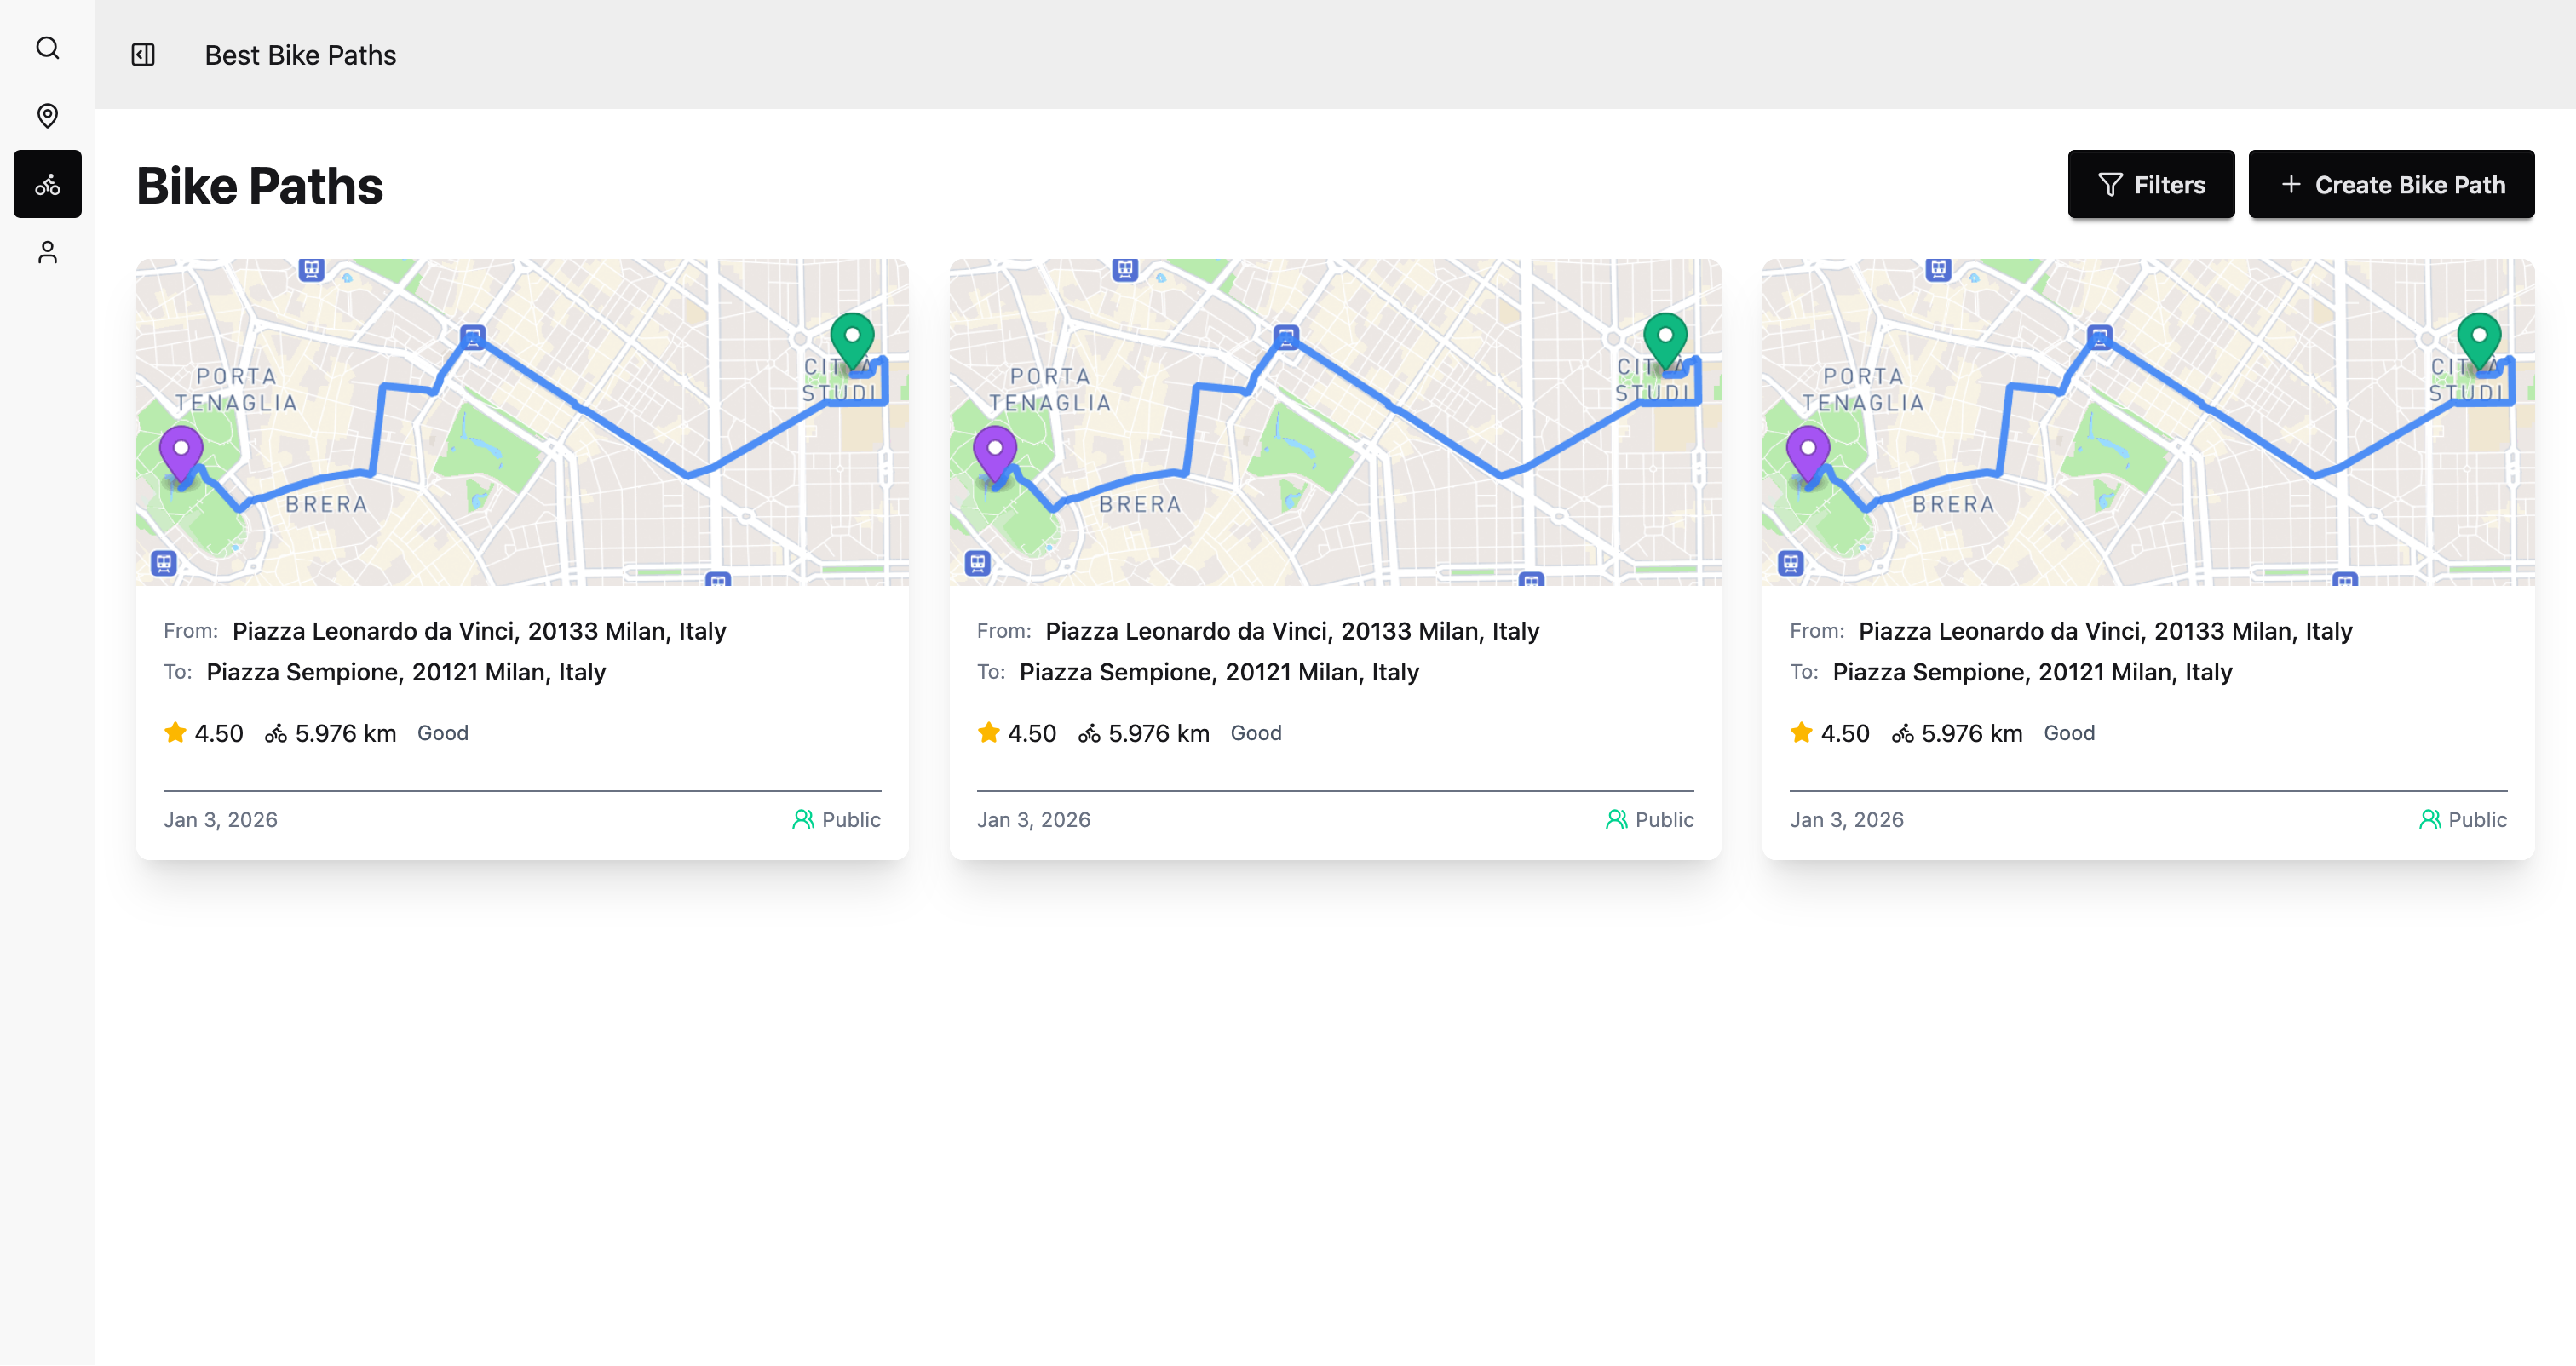
\includegraphics[width=\linewidth]{DD/images/ui-bike-paths.png}
    \caption{Bike Paths}
    \label{fig:ui-bike-paths}
\end{figure}
\begin{figure}[h!]
    \centering
        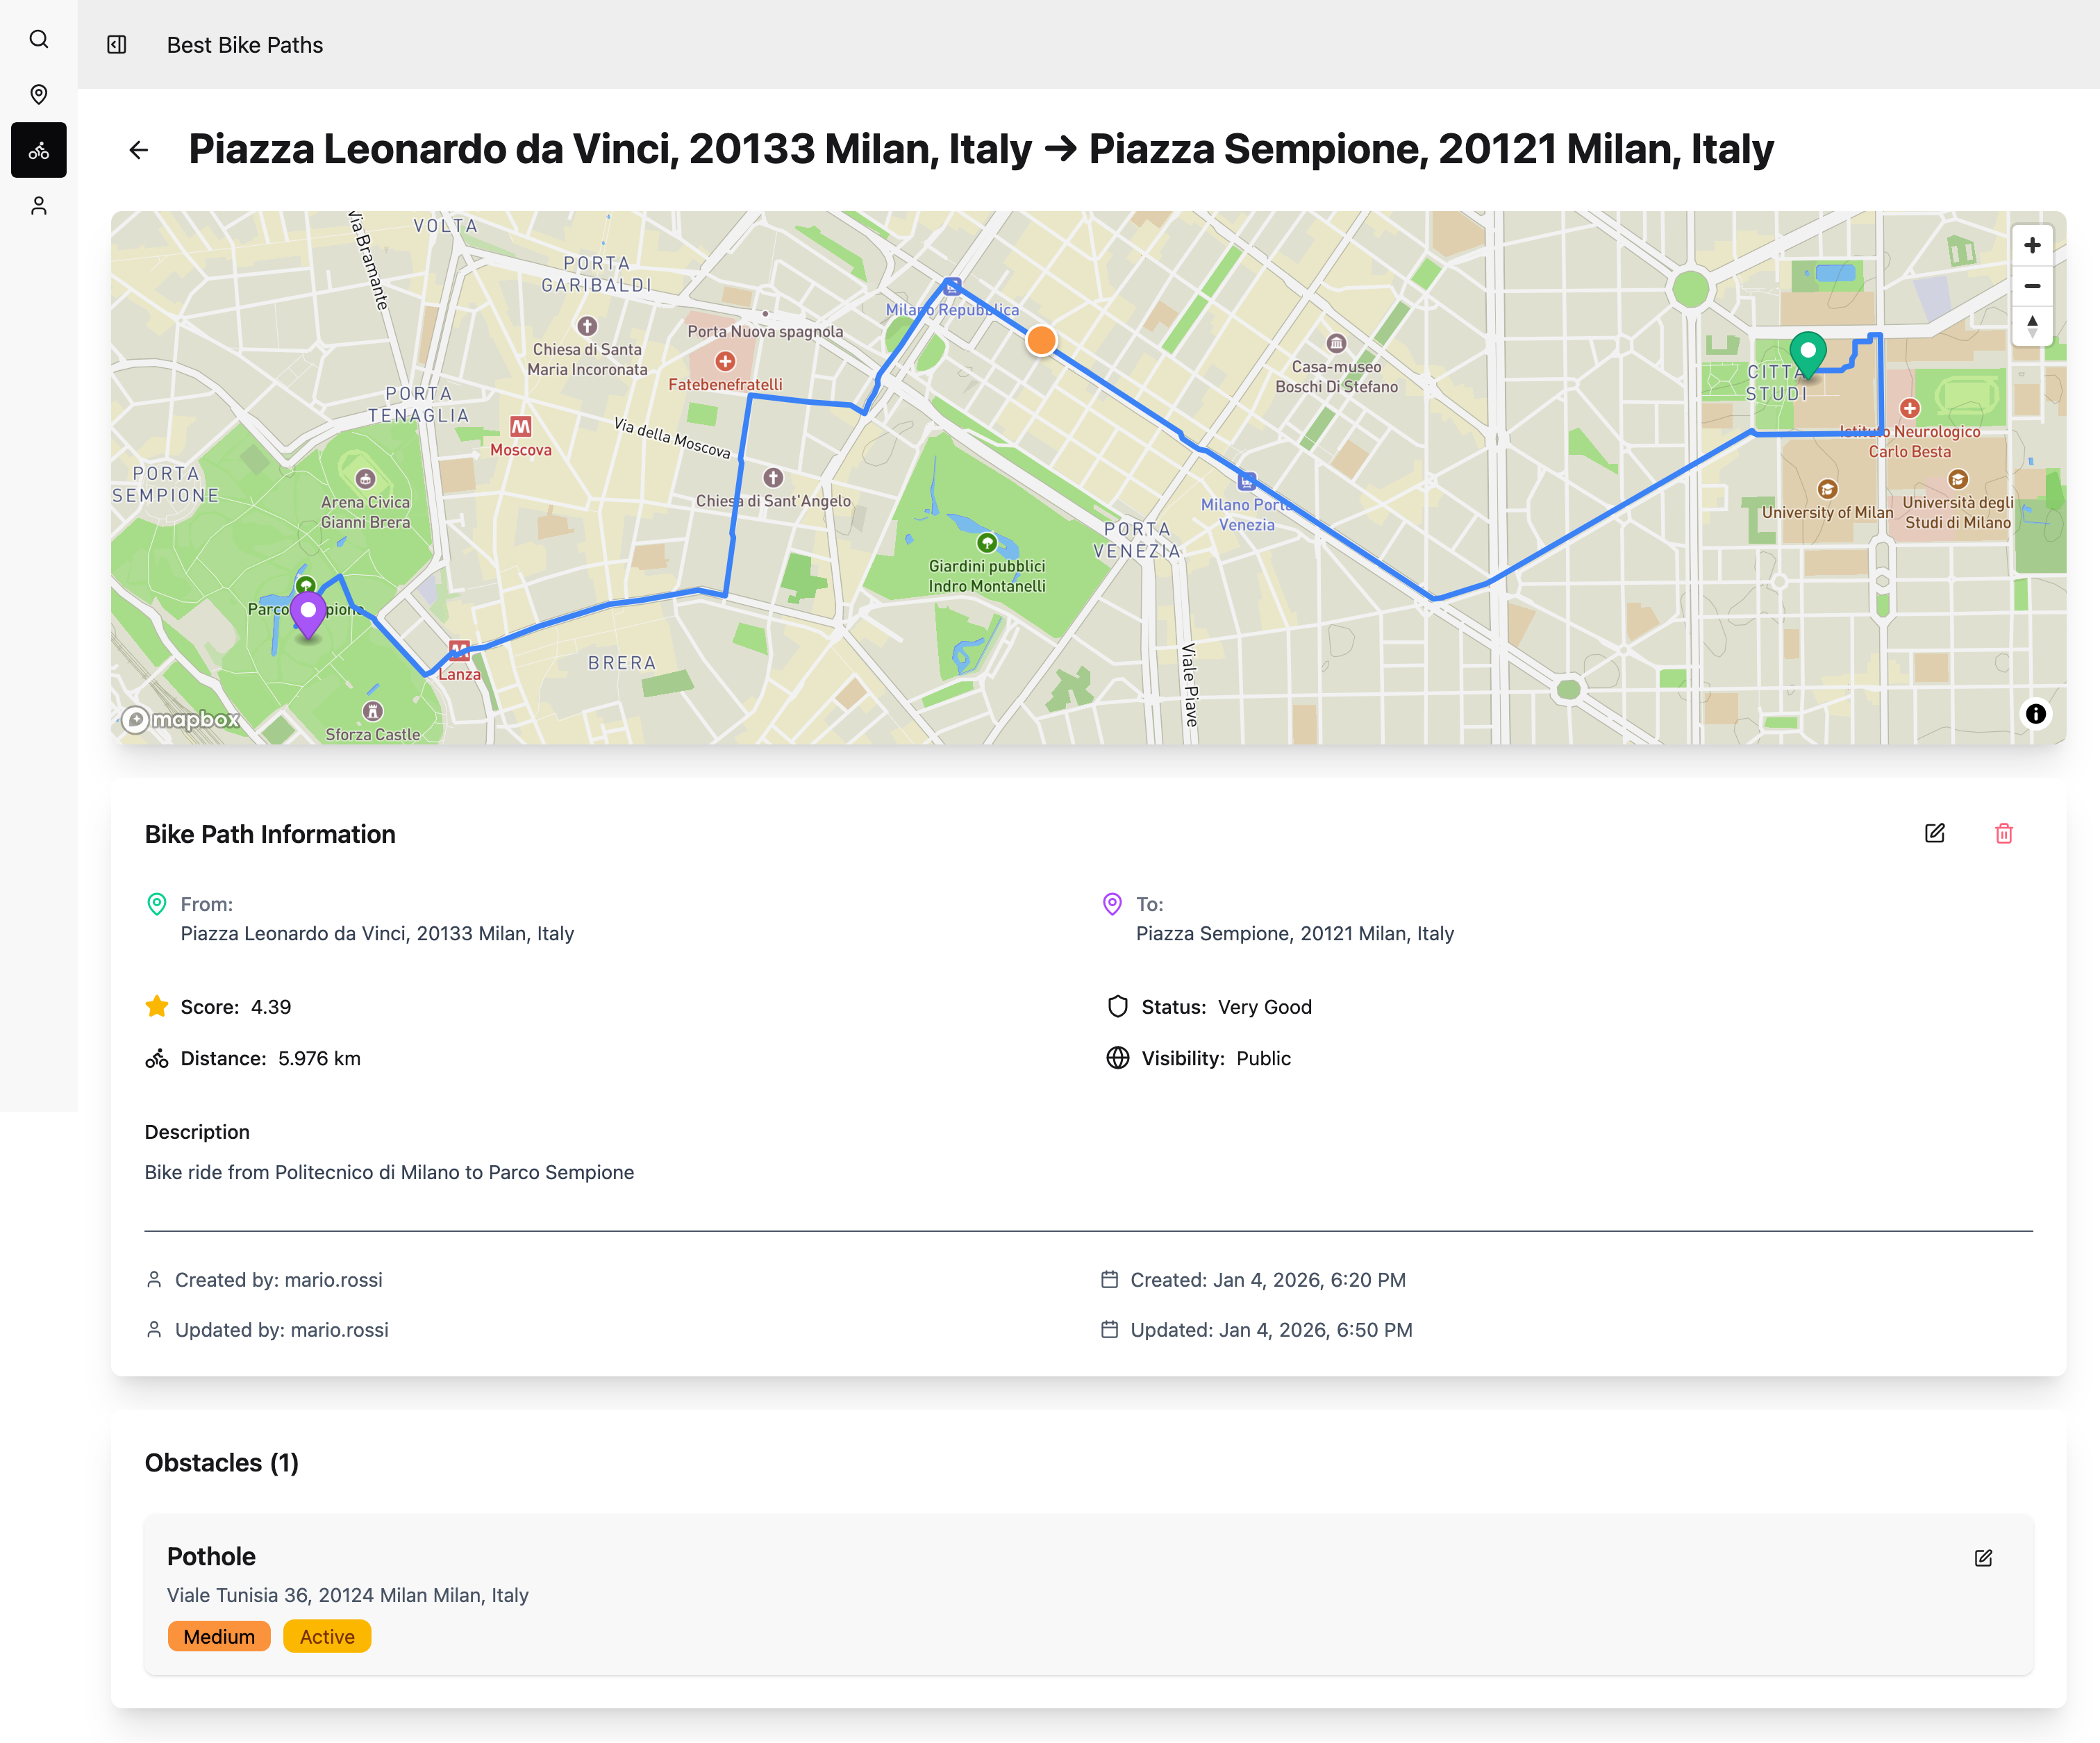
\includegraphics[width=\linewidth]{DD/images/ui-bike-path-detail.png}
    \caption{Bike Path Detail}
    \label{fig:ui-bike-path-detail}
\end{figure}
\begin{figure}[h!]
    \centering
        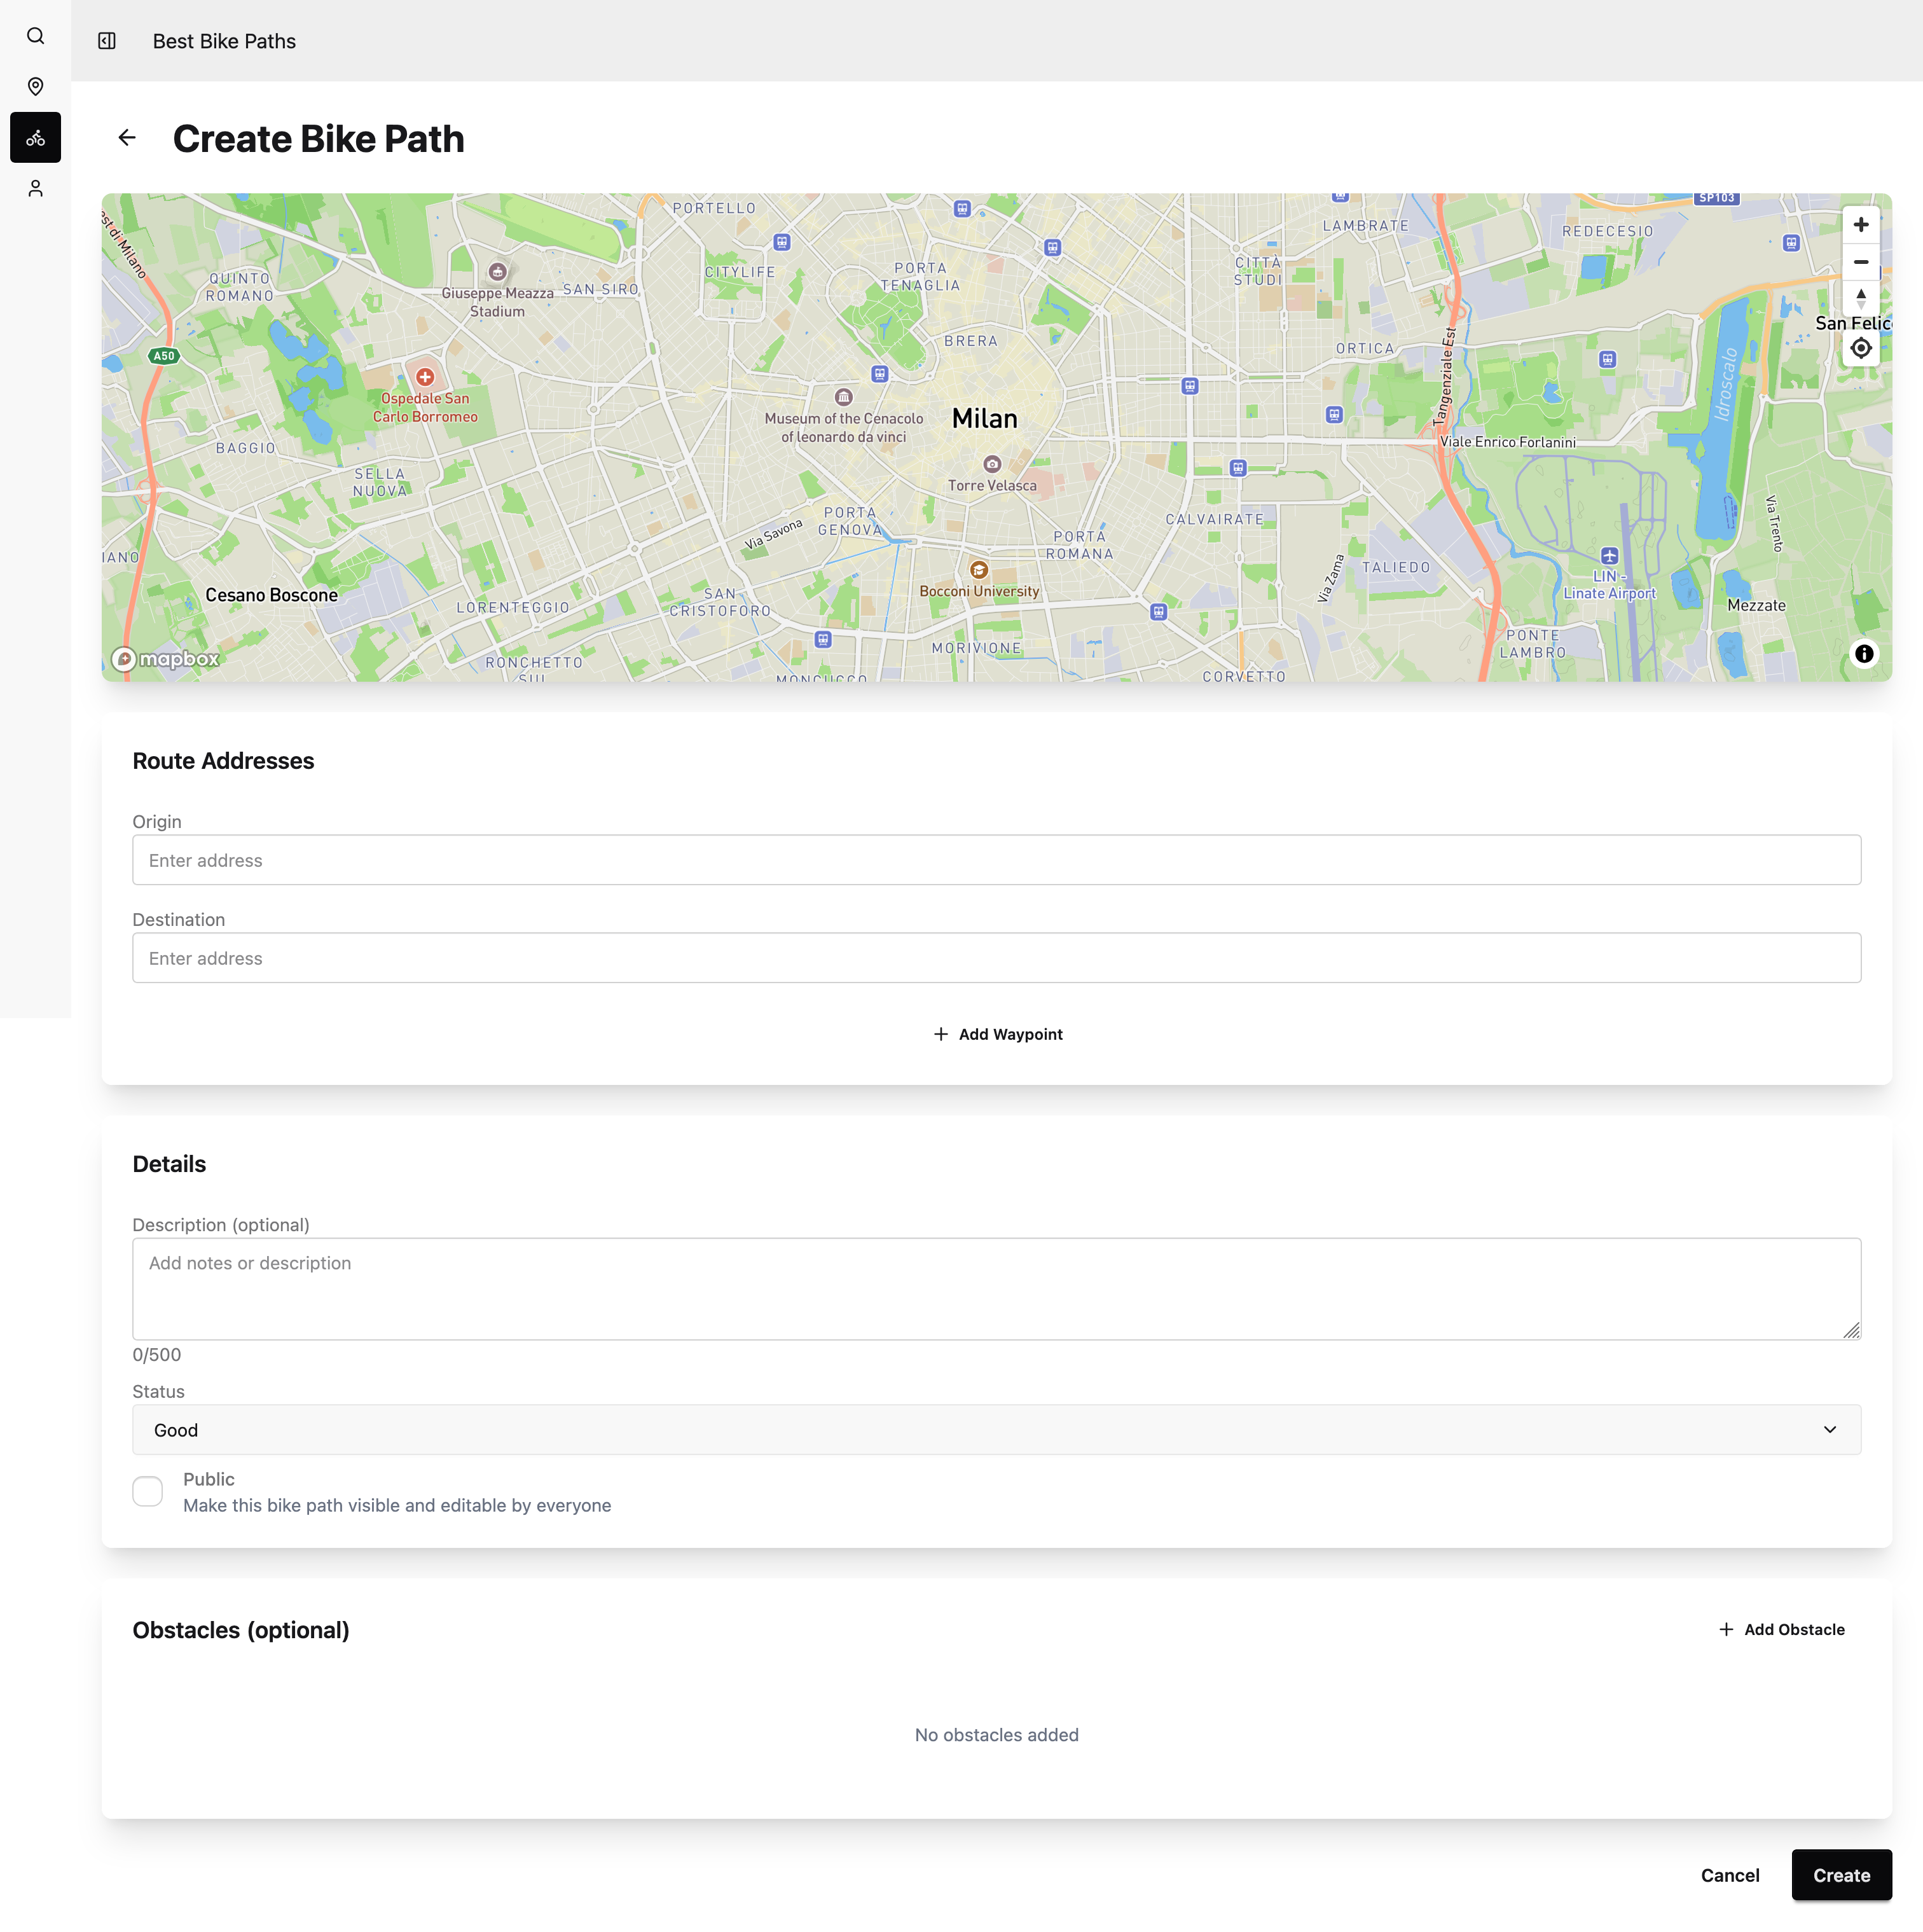
\includegraphics[width=\linewidth]{DD/images/ui-create-bike-path.png}
    \caption{Bike Path Create Manual}
    \label{fig:ui-create-bike-path}
\end{figure}

\subsubsection{Profile Management}
The authentication and profile section allows managing the user account through three main views. The Login view presents a centered form with fields for email and password, a "Login" button and a "Don't have an account? Register" link to move to the registration. The Register view shows a similar form with additional fields for first name, last name and username, a "Register" button and an "Already have an account? Login" link to return to the login. The Profile view displays the user data (first name, last name, username, email) in read-only mode with "Edit" and "Logout" buttons in the main interface. Clicking on "Edit", the profile switches to edit mode transforming the information into editable fields, including an optional field to change the password, with "Cancel" and "Save" buttons to confirm or cancel the modifications. A "Delete Account" button allows definitively deleting the account through a confirmation modal.
\begin{figure}[h!]
    \centering
        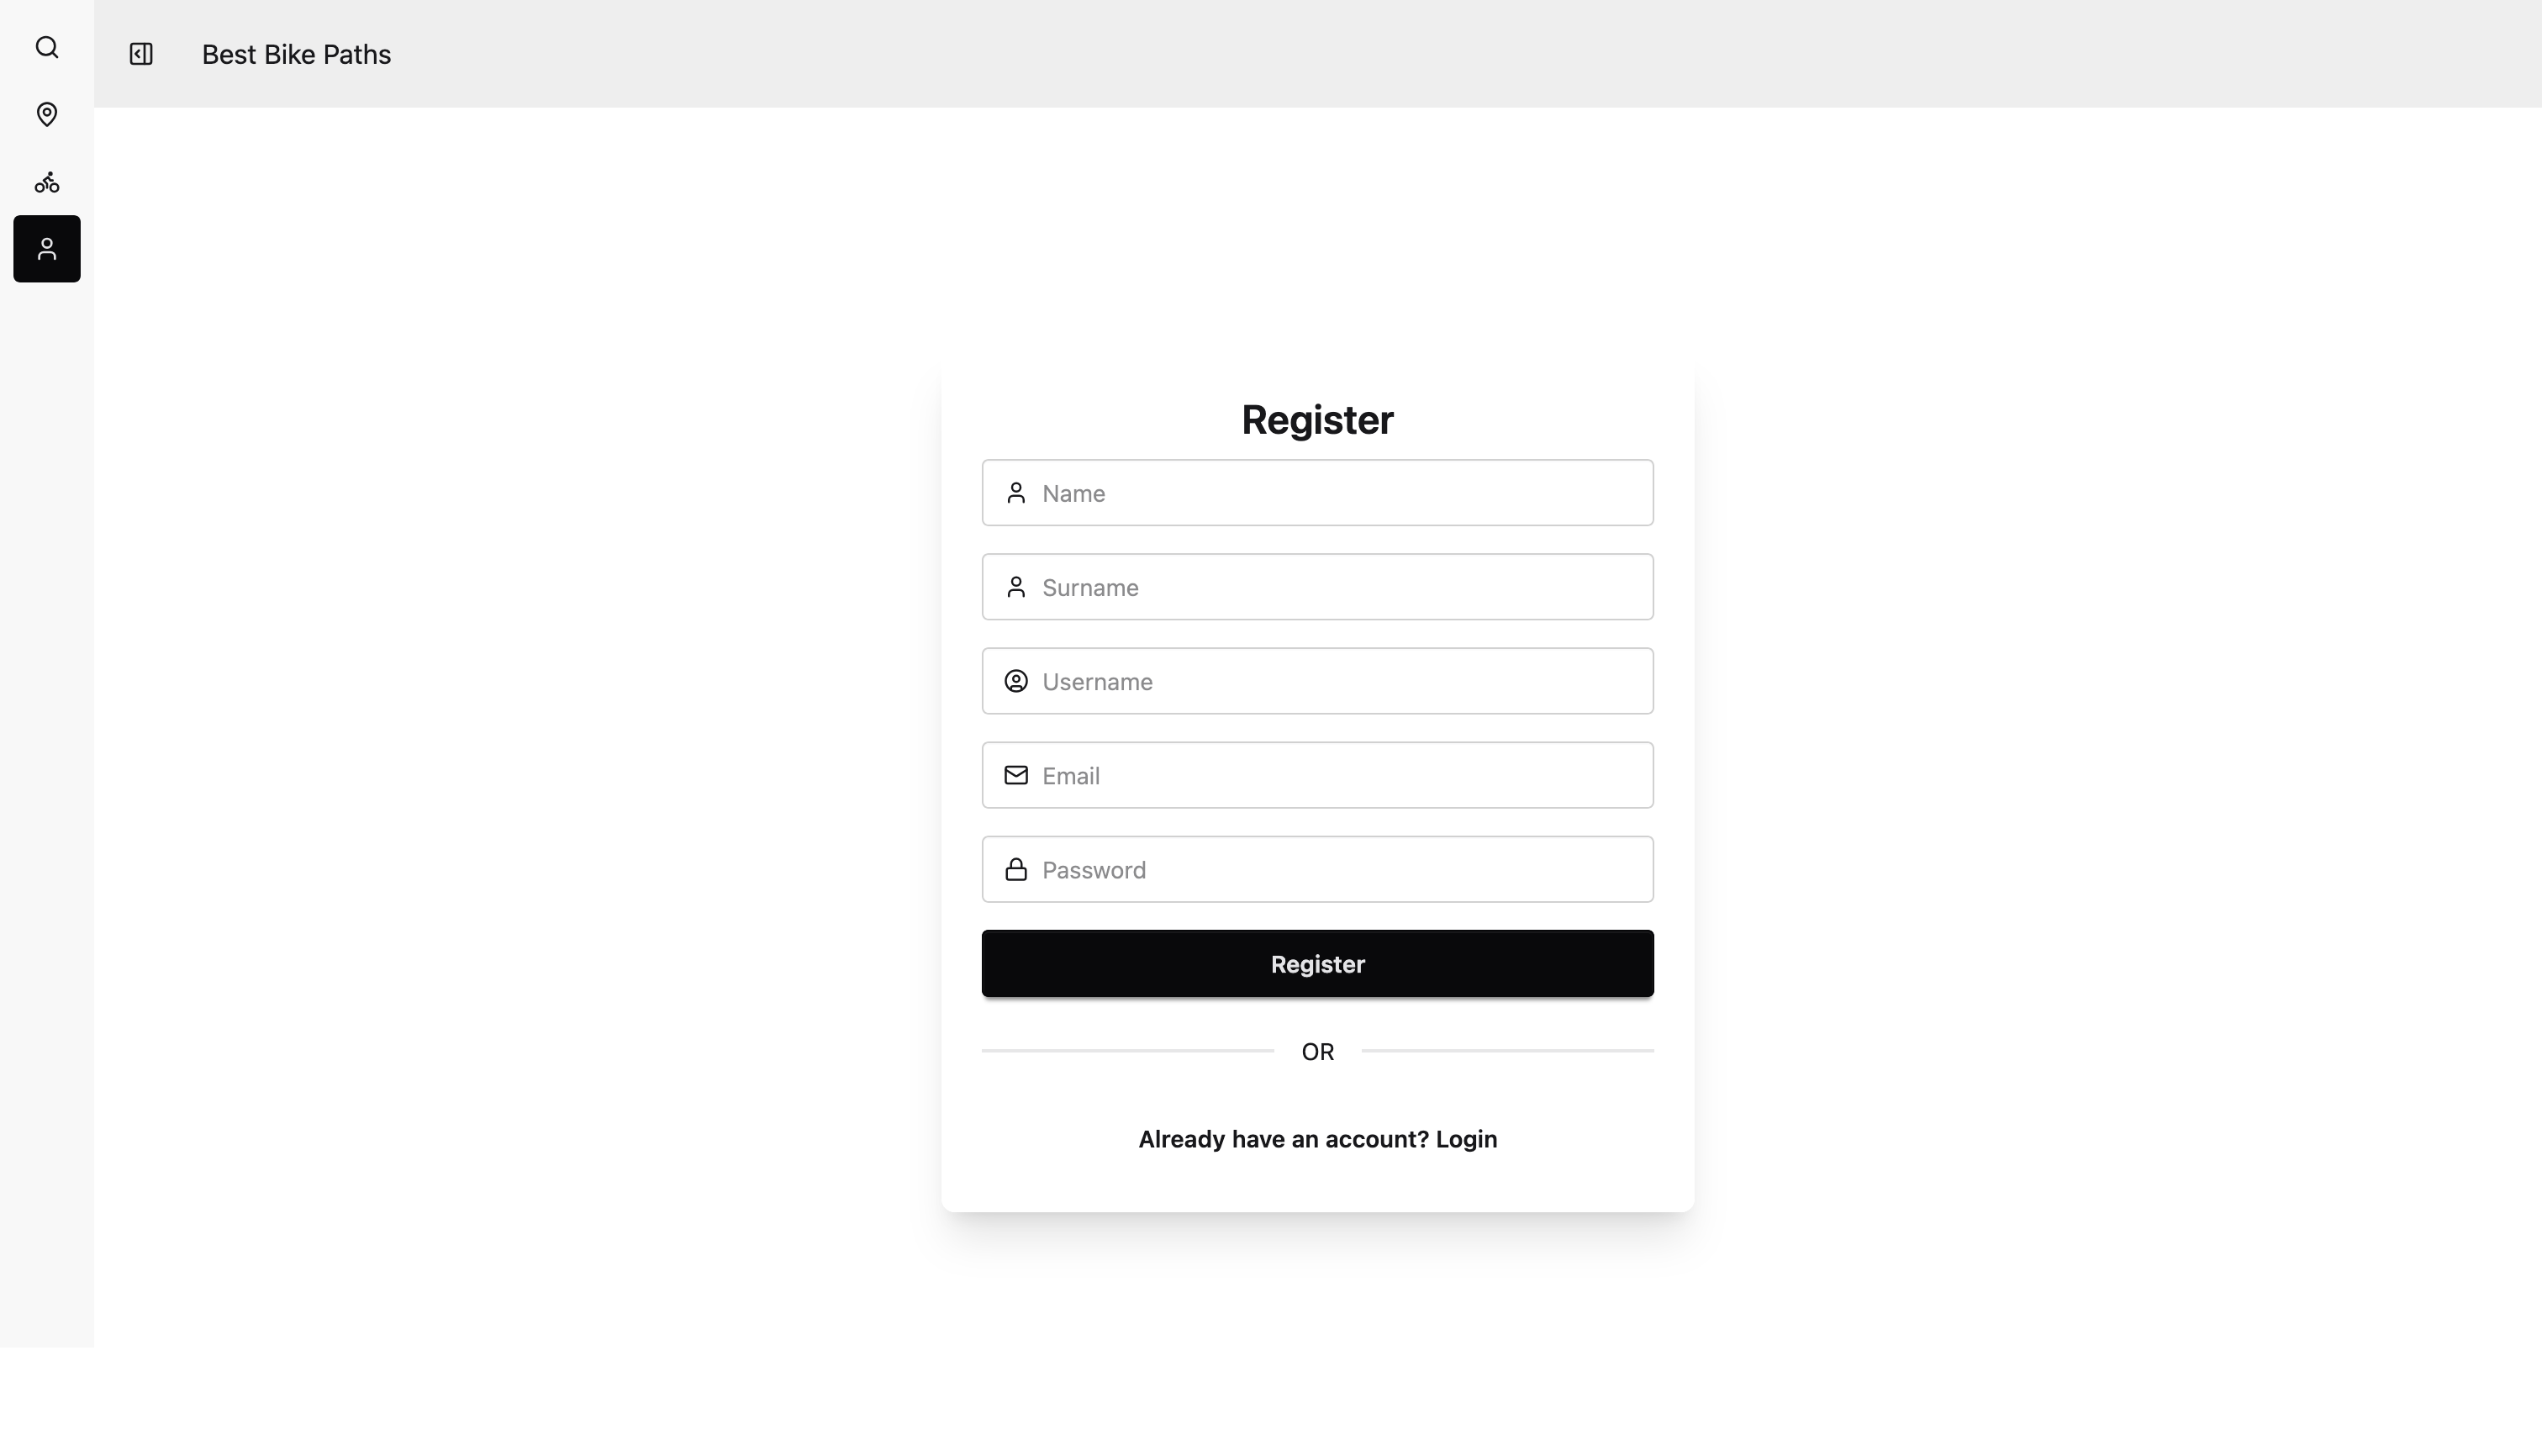
\includegraphics[width=\linewidth]{DD/images/ui-register.png}
    \caption{Register}
    \label{fig:ui-register}
\end{figure}
\begin{figure}[h!]
    \centering
        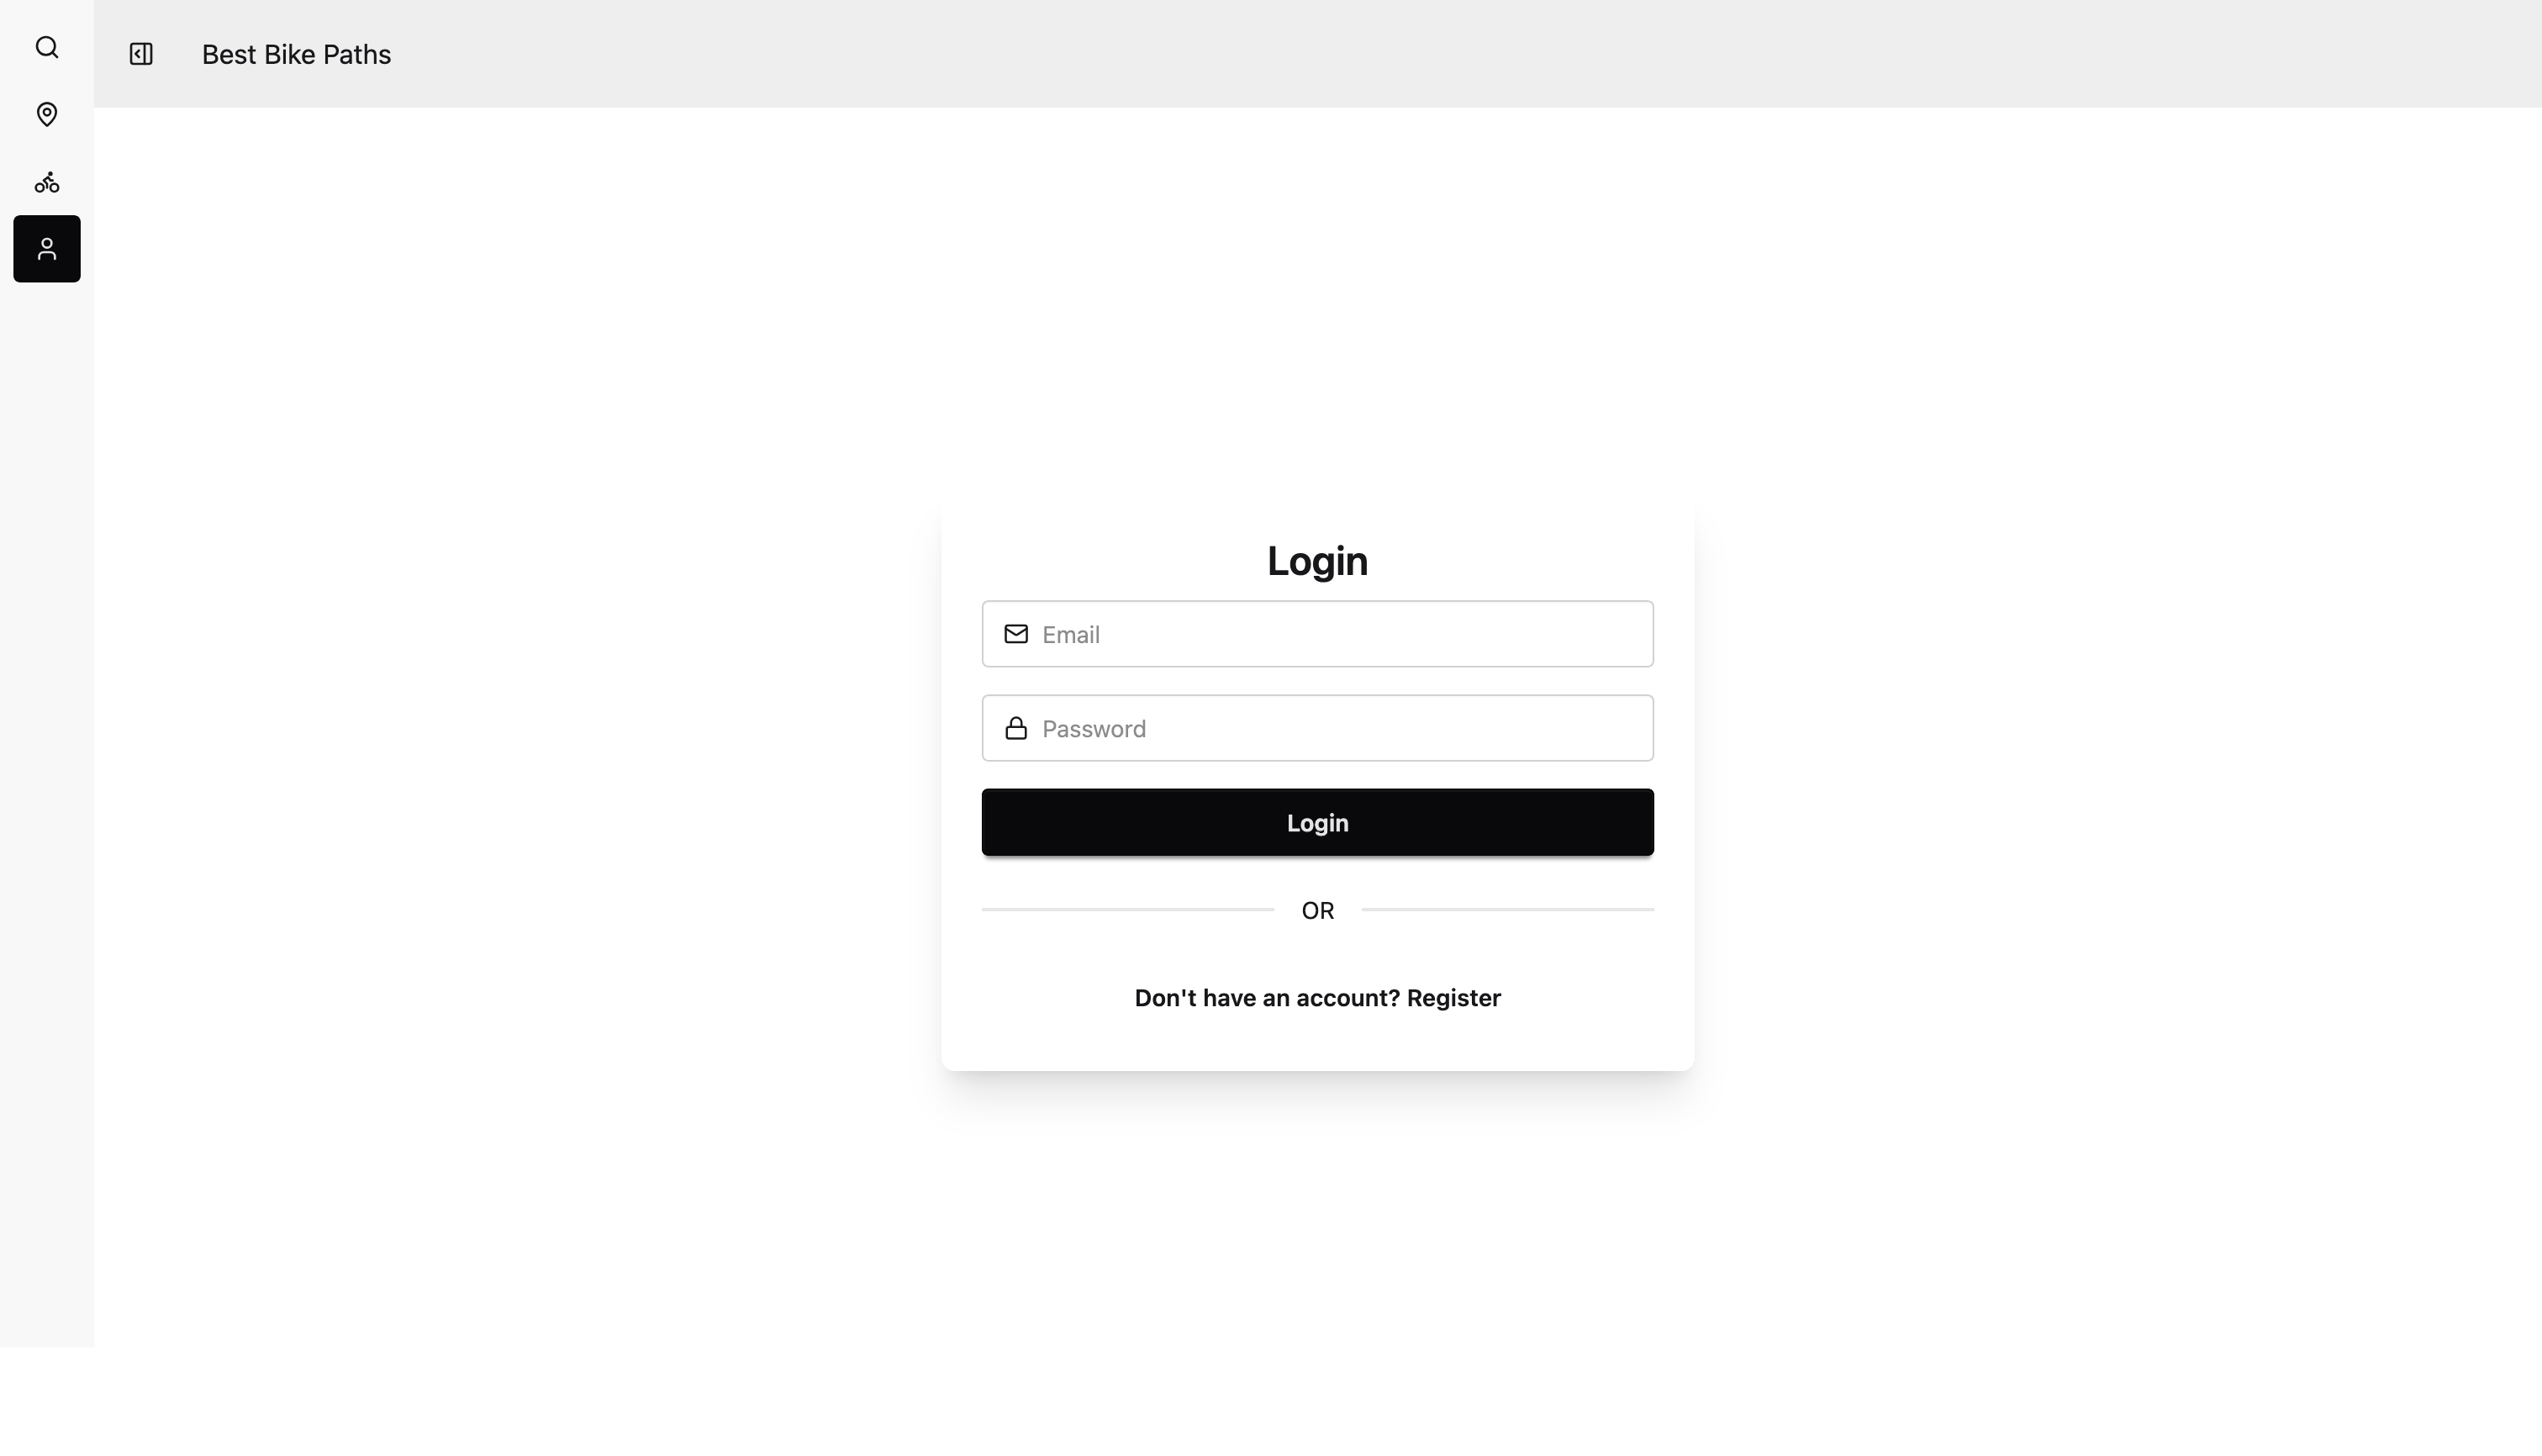
\includegraphics[width=\linewidth]{DD/images/ui-login.png}
    \caption{Login}
    \label{fig:ui-login}
\end{figure}
\begin{figure}[h!]
    \centering
        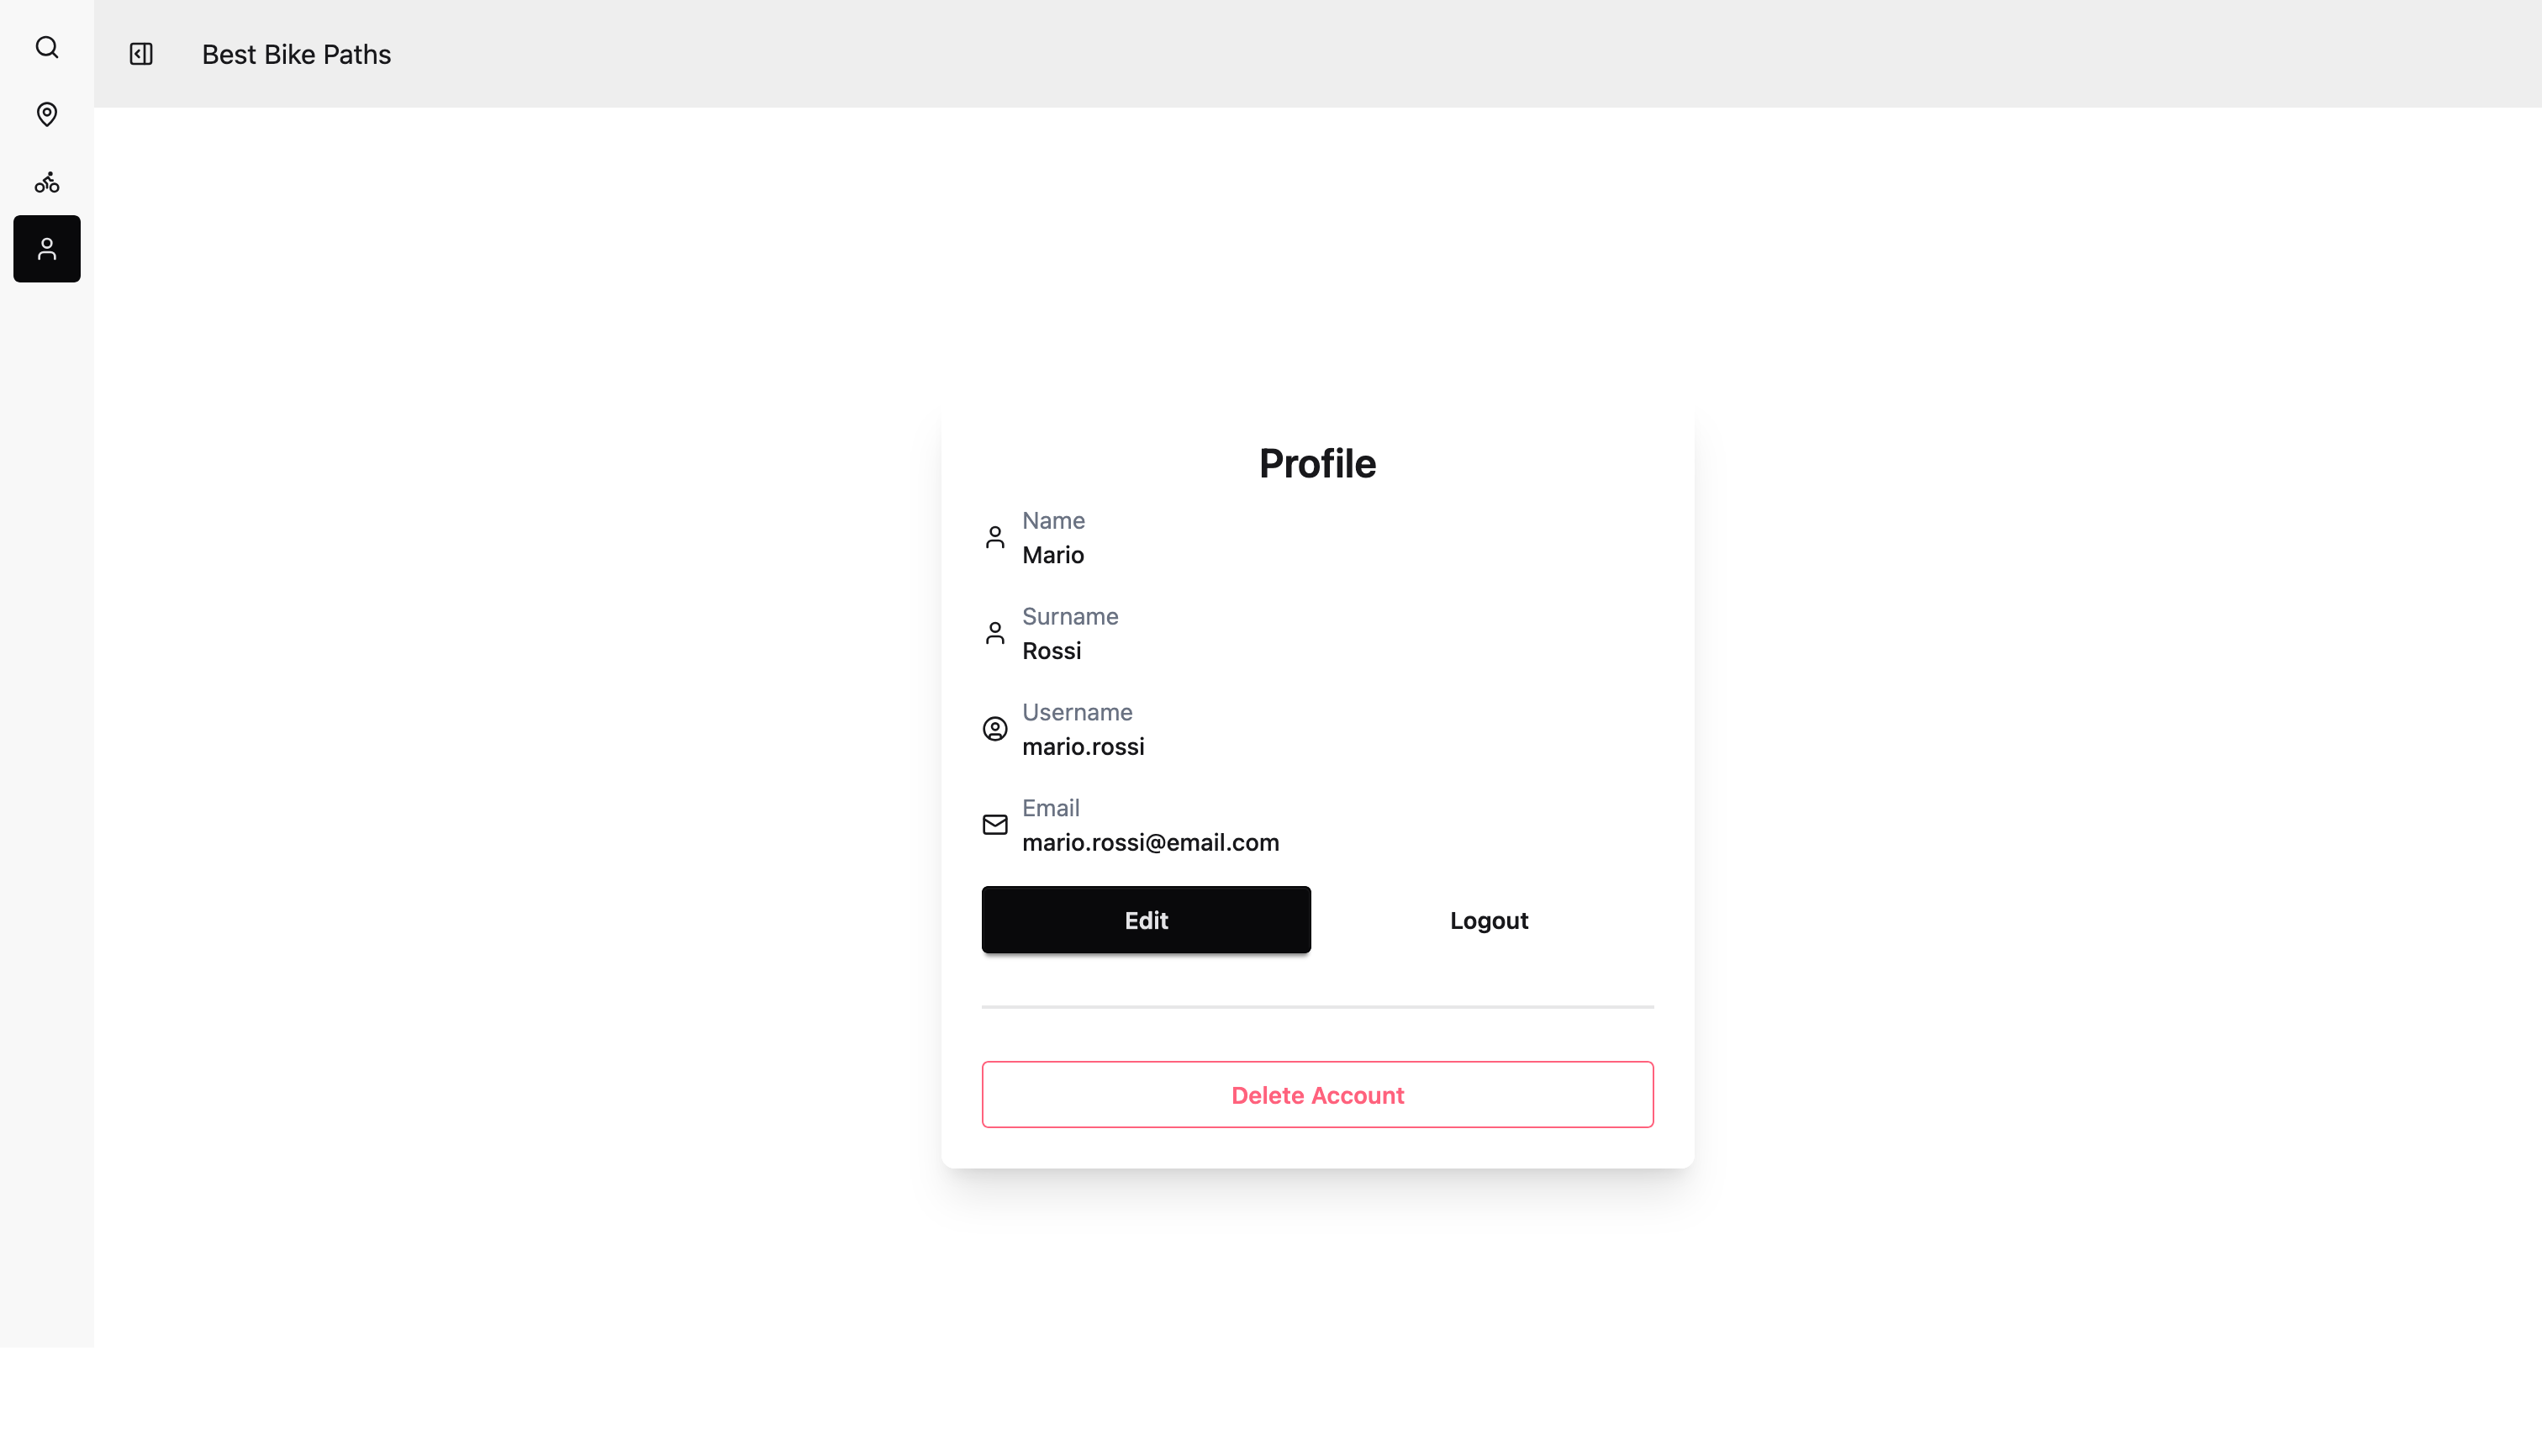
\includegraphics[width=\linewidth]{DD/images/ui-profile.png}
    \caption{Profile}
    \label{fig:ui-profile}
\end{figure}

\subsection{Mobile App}
The BBP mobile application, developed in Flutter, offers all the functionalities of the web version adapted for the use on mobile devices. The interface has been optimized for vertical screens and for touch interaction, guaranteeing a fluid use experience even during movements.
The main navigation occurs through a fixed dock positioned in the lower part of the screen. This bar contains four icons that allow accessing rapidly the main sections of the application:
\begin{itemize}
    \item \textbf{Magnifying glass}: accesses the Bike Path Finder section to search available routes
    \item \textbf{Geographic pin}: shows the Trips section with the history of registered trips
    \item \textbf{Bicycle}: opens the Bike Paths section to manage the created routes
    \item \textbf{User profile}: allows visualizing and modifying the personal data
\end{itemize}
The mobile screens maintain the same functionalities of the web version, but with a reorganized layout to exploit at best the available vertical space. The cards of the routes and of the trips are presented in a vertically scrollable list, each one with a preview of the map reduced but always readable. The insertion and modification forms have been adapted to facilitate the typing on virtual keyboard, with larger and spaced controls to guarantee a greater precision in the input.
The distinctive characteristic of the mobile application is the integration with the sensors of the device. The GPS is used for the real-time registration of the trips, tracing automatically the route followed by the user during the cycling. During the registration of a trip, the app visualizes a live map with the current position and the traced route until that moment.
\begin{figure}[h!]
    \centering
        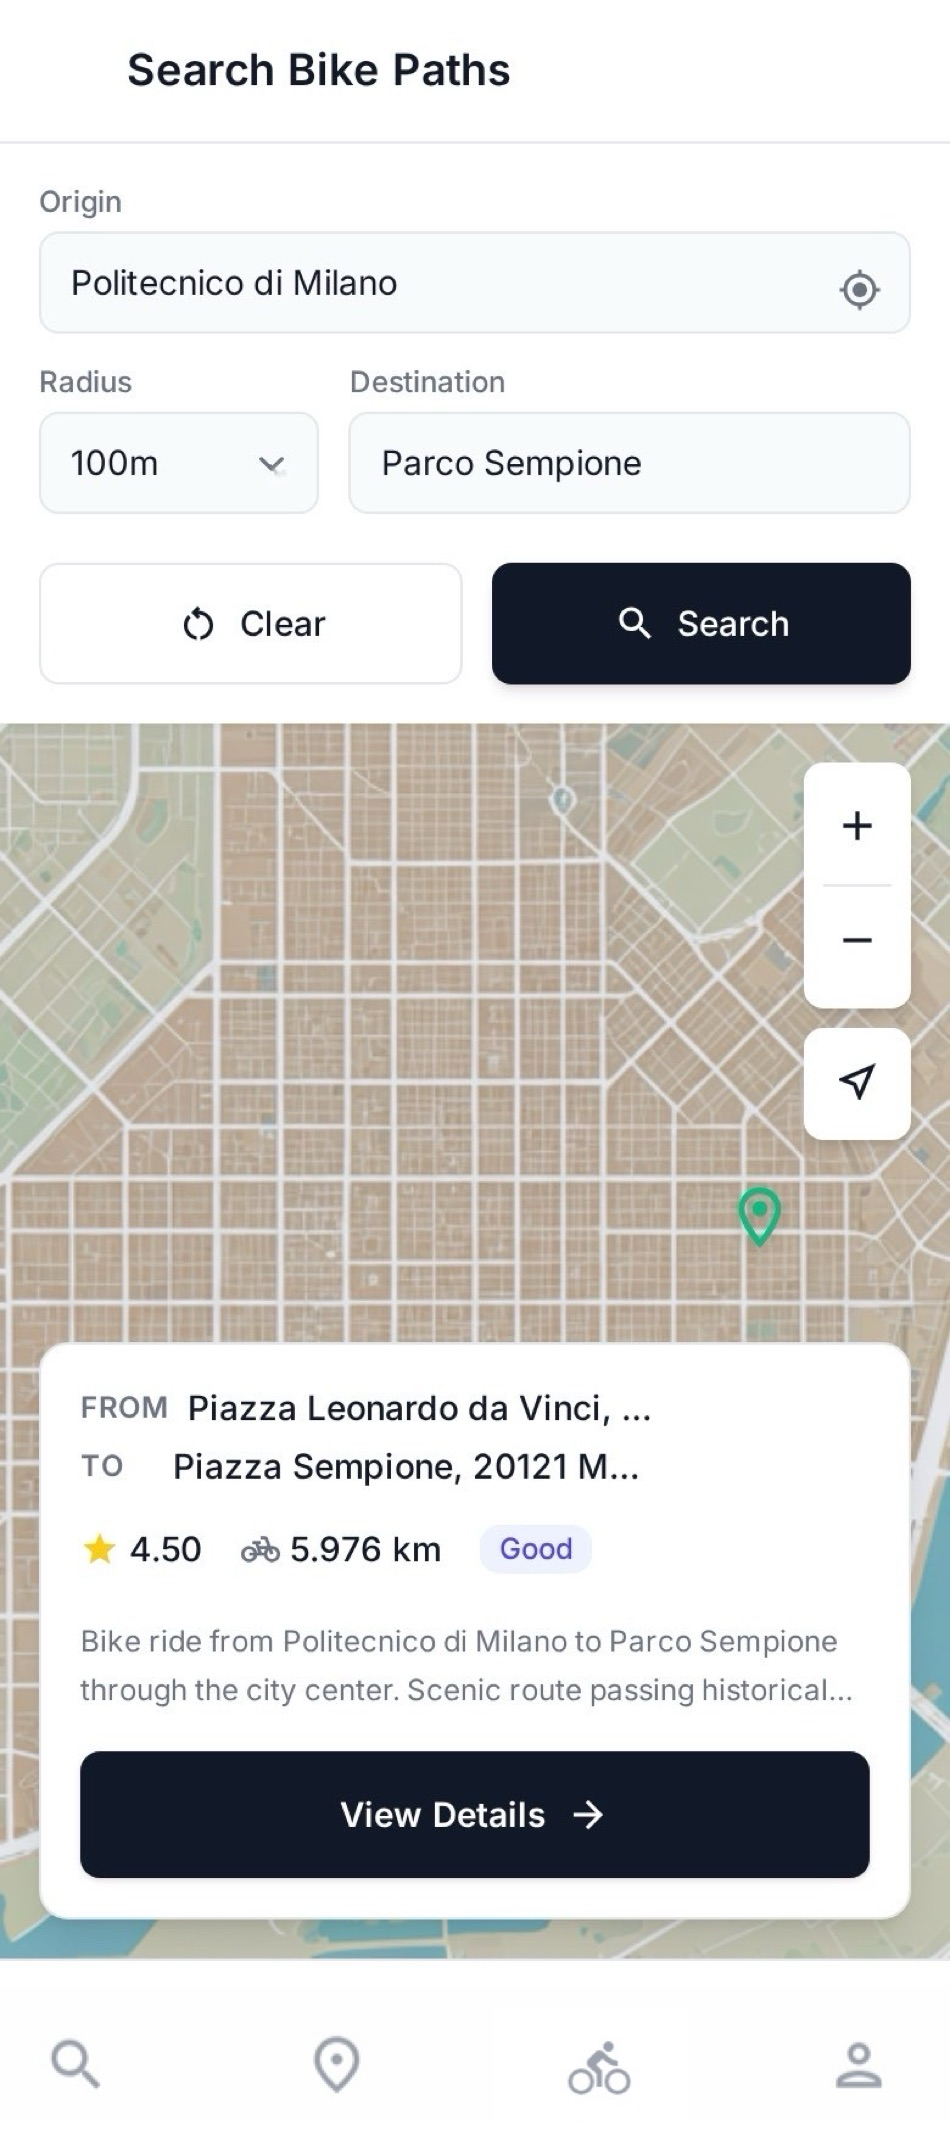
\includegraphics[width=\linewidth]{DD/images/ui-finder-mobile.jpg}
    \caption{Bike Path Finder}
    \label{fig:ui-finder-mobile}
\end{figure}
\begin{figure}[h!]
    \centering
        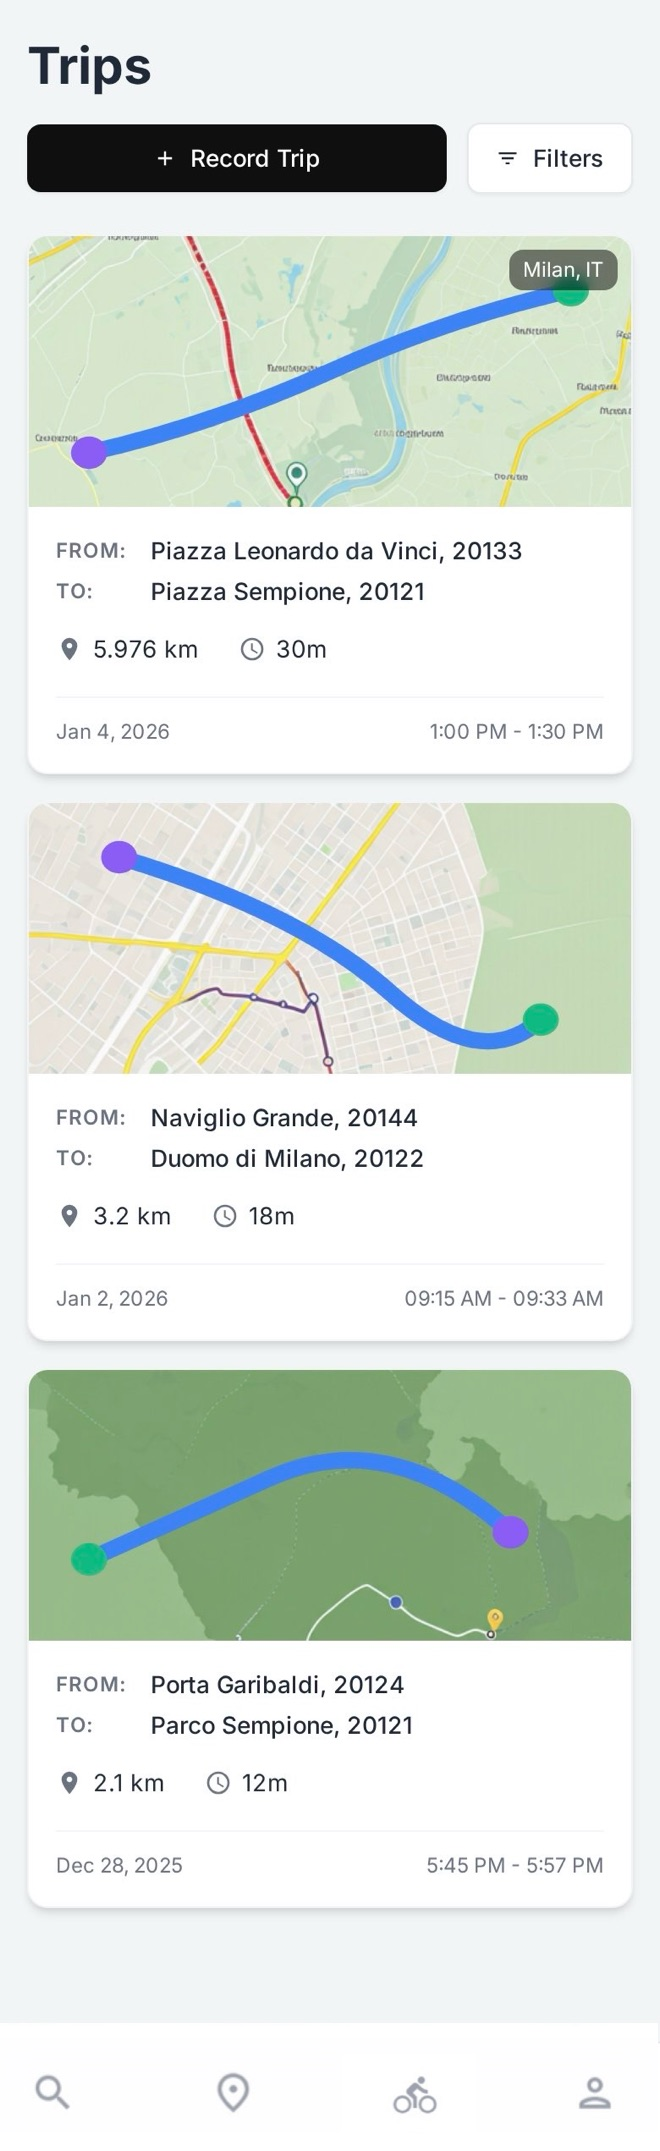
\includegraphics[width=\linewidth]{DD/images/ui-trips-mobile.jpg}
    \caption{Trips}
    \label{fig:ui-trips-mobile}
\end{figure}
\begin{figure}[h!]
    \centering
        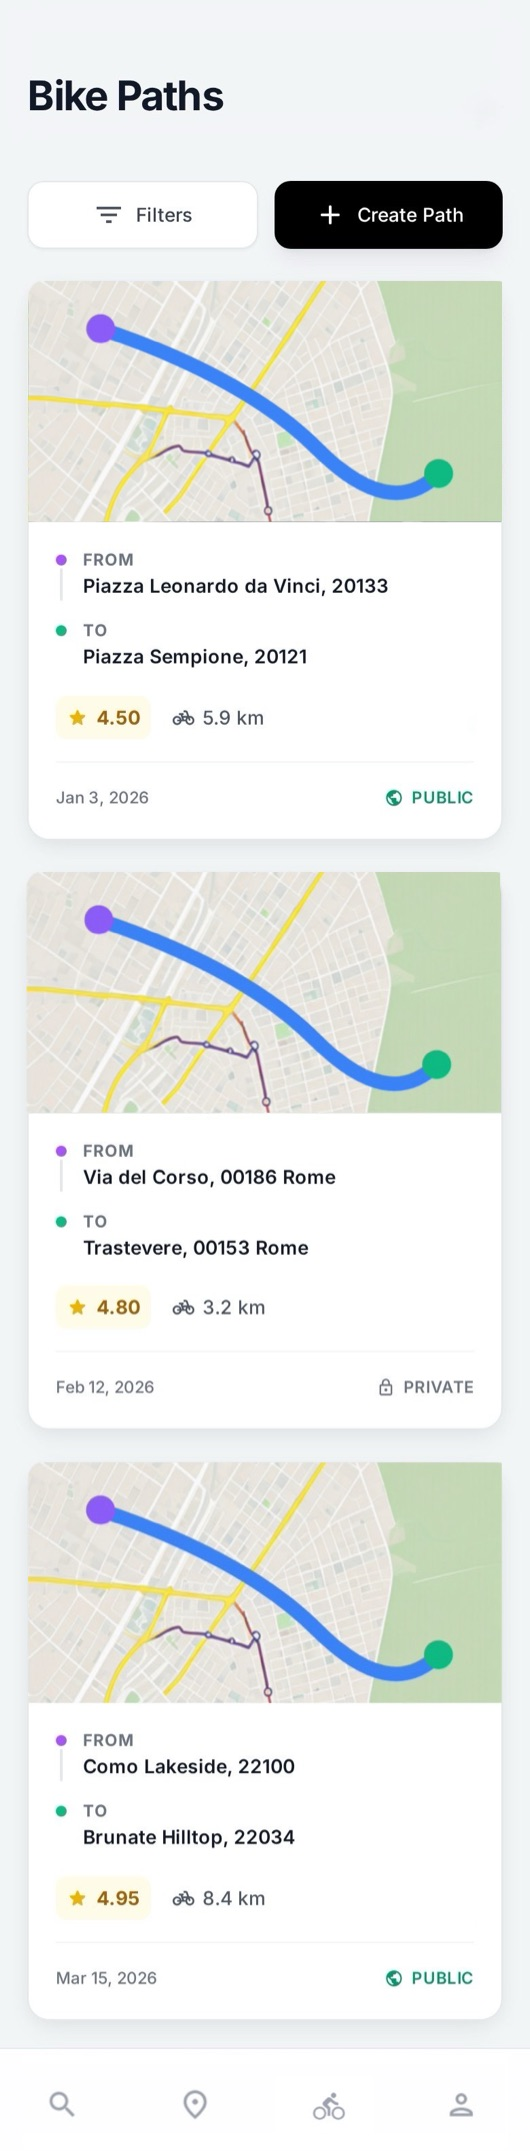
\includegraphics[width=\linewidth]{DD/images/ui-bike-paths-mobile.jpg}
    \caption{Bike Paths}
    \label{fig:ui-bike-paths-mobile}
\end{figure}
\begin{figure}[h!]
    \centering
        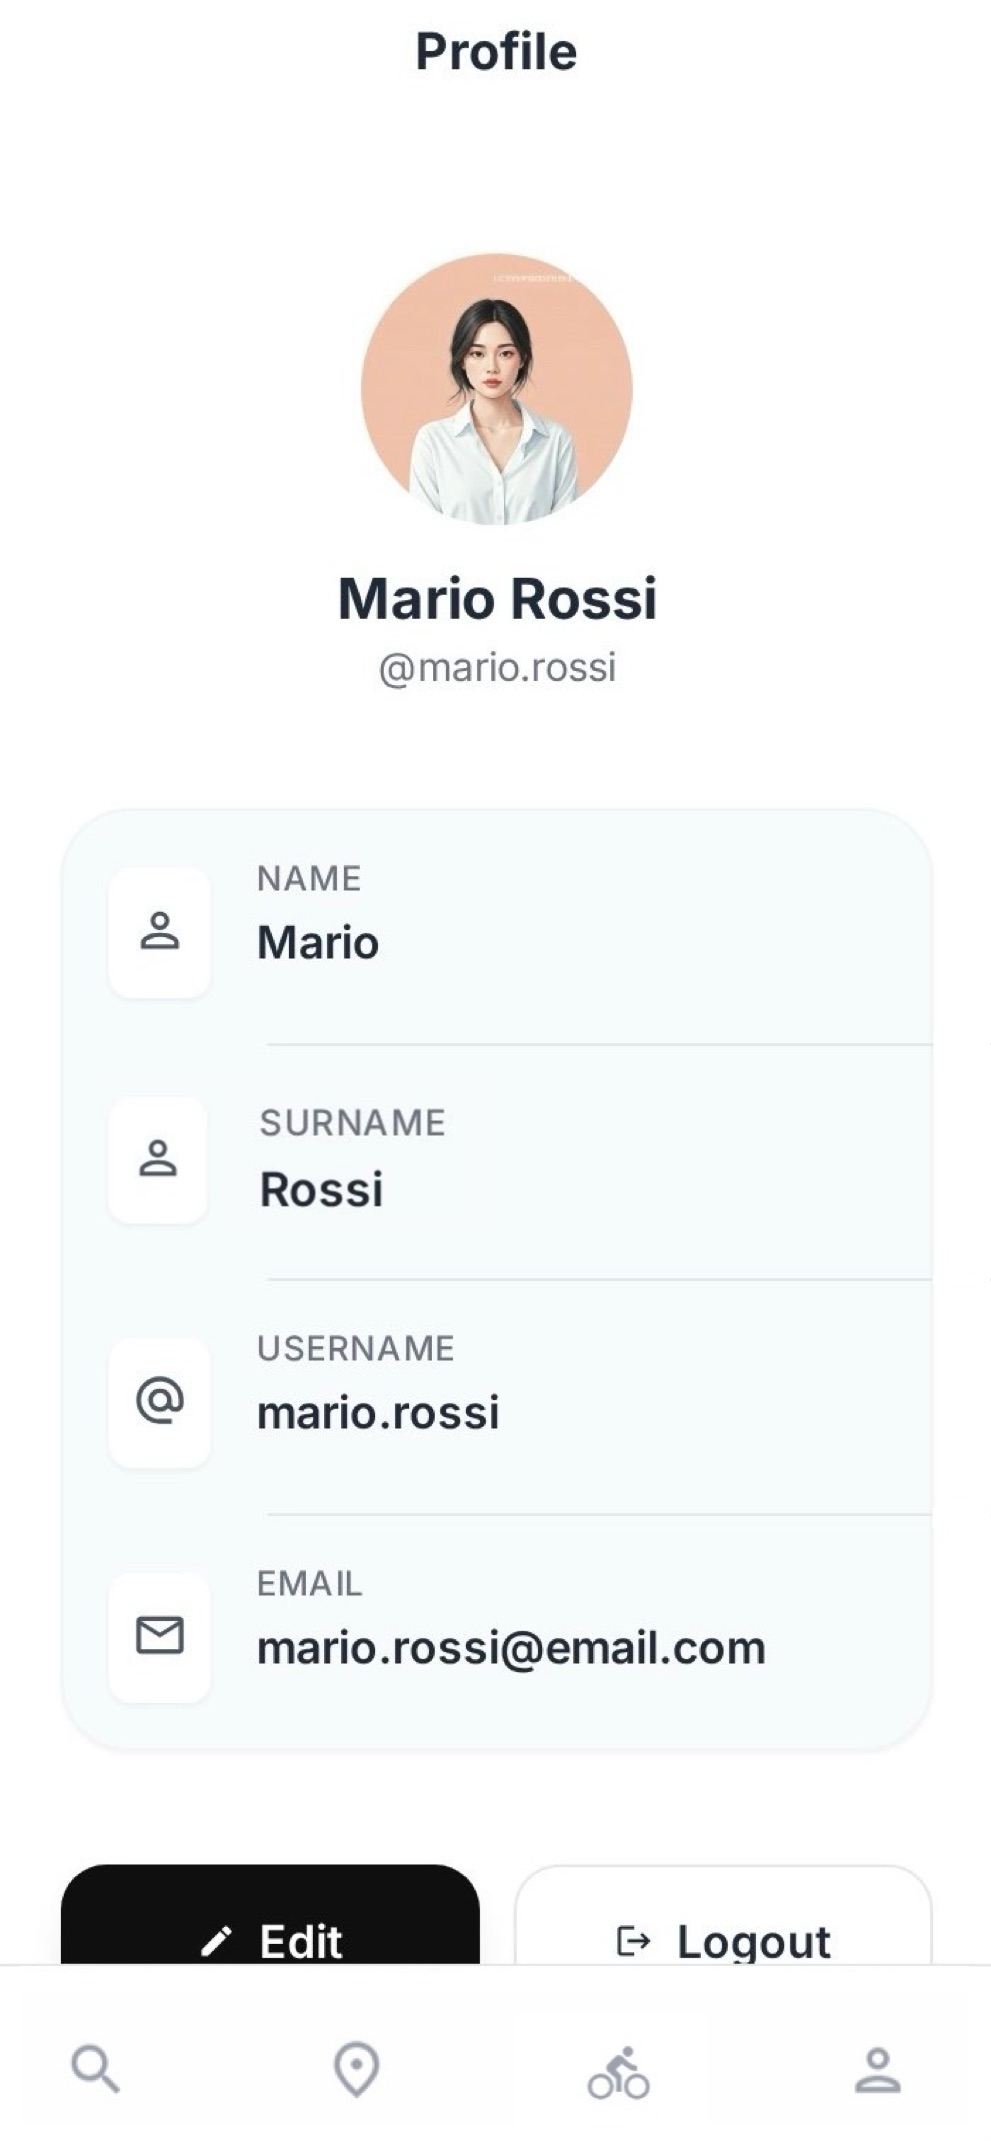
\includegraphics[width=\linewidth]{DD/images/ui-profile-mobile.jpg}
    \caption{Profile}
    \label{fig:ui-profile-mobile}
\end{figure}